\documentclass[11pt,twoside]{report}

%%%%%%%%%%%%%%%%%%%%%%%%%%%%%%%%%%%%%%%%%%%%%%%%%%%%%%%%%%%%%%%%%%%%%%%%%%%%%

% Definitions for the title page
% Edit these to provide the correct information
% e.g. \newcommand{\reportauthor}{Timothy Kimber}

\newcommand{\reporttitle}{Combining Autoencoding and Classifying Neural Networks for Joint Facial Action Unit Recognition}
\newcommand{\reportauthor}{Luka Milic}
\newcommand{\supervisor}{Sebastian Kaltwang and Maja Pantic}
\newcommand{\degreetype}{Computing Science}
\newcommand{\networkI}{conv 0}
\newcommand{\networkII}{conv 1}
\newcommand{\networkIII}{conv 2}
\newcommand{\networkIV}{conv 3}

%%%%%%%%%%%%%%%%%%%%%%%%%%%%%%%%%%%%%%%%%%%%%%%%%%%%%%%%%%%%%%%%%%%%%%%%%%%%%
% load some definitions and default packages
%%%%%%%%%%%%%%%%%%%%%%%%%%%%%%%%%%%%%%%%%
% University Assignment Title Page 
% LaTeX Template
% Version 1.0 (27/12/12)
%
% This template has been downloaded from:
% http://www.LaTeXTemplates.com
%
% Original author:
% WikiBooks (http://en.wikibooks.org/wiki/LaTeX/Title_Creation)
%
% License:
% CC BY-NC-SA 3.0 (http://creativecommons.org/licenses/by-nc-sa/3.0/)
% 
%
%%%%%%%%%%%%%%%%%%%%%%%%%%%%%%%%%%%%%%%%%
%----------------------------------------------------------------------------------------
%	PACKAGES AND OTHER DOCUMENT CONFIGURATIONS
%----------------------------------------------------------------------------------------
\usepackage[a4paper,hmargin=2.8cm,vmargin=2.0cm,includeheadfoot]{geometry}
\usepackage{textpos}
\usepackage{natbib} % for bibliography
\usepackage{tabularx,longtable,multirow,subfigure,caption}%hangcaption
\usepackage{fncylab} %formatting of labels
\usepackage{fancyhdr} % page layout
\usepackage{url} % URLs
\usepackage[english]{babel}
\usepackage{amsmath}
\usepackage{graphicx}
\usepackage{dsfont}
\usepackage{epstopdf} % automatically replace .eps with .pdf in graphics
\usepackage{backref} % needed for citations
\usepackage{array}
\usepackage{latexsym}
\usepackage[pdftex,pagebackref,hypertexnames=false,colorlinks]{hyperref} % provide links in pdf

\hypersetup{pdftitle={},
  pdfsubject={}, 
  pdfauthor={},
  pdfkeywords={}, 
  pdfstartview=FitH,
  pdfpagemode={UseOutlines},% None, FullScreen, UseOutlines
  bookmarksnumbered=true, bookmarksopen=true, colorlinks,
    citecolor=black,%
    filecolor=black,%
    linkcolor=black,%
    urlcolor=black}

\usepackage[all]{hypcap}


%\usepackage{color}
%\usepackage[tight,ugly]{units}
%\usepackage{float}
%\usepackage{tcolorbox}
%\usepackage[colorinlistoftodos]{todonotes}
% \usepackage{ntheorem}
% \theoremstyle{break}
% \newtheorem{lemma}{Lemma}
% \newtheorem{theorem}{Theorem}
% \newtheorem{remark}{Remark}
% \newtheorem{definition}{Definition}
% \newtheorem{proof}{Proof}


%%% Default fonts
\renewcommand*{\rmdefault}{bch}
\renewcommand*{\ttdefault}{cmtt}



%%% Default settings (page layout)
\setlength{\parindent}{0em}  % indentation of paragraph

\setlength{\headheight}{14.5pt}
\pagestyle{fancy}
\renewcommand{\chaptermark}[1]{\markboth{\chaptername\ \thechapter.\ #1}{}} 

\fancyfoot[ER,OL]{\sffamily\textbf{\thepage}}%Page no. in the left on odd pages and on right on even pages
\fancyfoot[OC,EC]{\sffamily }
\renewcommand{\headrulewidth}{0.1pt}
\renewcommand{\footrulewidth}{0.1pt}
\captionsetup{margin=10pt,font=small,labelfont=bf}


%--- chapter heading

\def\@makechapterhead#1{%
  \vspace*{10\p@}%
  {\parindent \z@ \raggedright \sffamily
    \interlinepenalty\@M
    \Huge\bfseries \thechapter \space\space #1\par\nobreak
    \vskip 30\p@
  }}

%---chapter heading for \chapter*  
\def\@makeschapterhead#1{%
  \vspace*{10\p@}%
  {\parindent \z@ \raggedright
    \sffamily
    \interlinepenalty\@M
    \Huge \bfseries  #1\par\nobreak
    \vskip 30\p@
  }}

\allowdisplaybreaks

% load some macros
% Here, you can define your own macros. Some examples are given below.

\newcommand{\R}[0]{\mathds{R}} % real numbers
\newcommand{\Z}[0]{\mathds{Z}} % integers
\newcommand{\N}[0]{\mathds{N}} % natural numbers
\newcommand{\C}[0]{\mathds{C}} % complex numbers
\renewcommand{\vec}[1]{{\boldsymbol{{#1}}}} % vector
\newcommand{\mat}[1]{{\boldsymbol{{#1}}}} % matrix


\date{September 2016}
\begin{document}

% load title page
% Last modification: 2015-08-17 (Marc Deisenroth)
\begin{titlepage}

\newcommand{\HRule}{\rule{\linewidth}{0.5mm}} % Defines a new command for the horizontal lines, change thickness here


%----------------------------------------------------------------------------------------
%	LOGO SECTION
%----------------------------------------------------------------------------------------


\includegraphics[width = 4cm]{./figures/imperial}\\[0.5cm]

\center % Center remainder of the page

%----------------------------------------------------------------------------------------
%	HEADING SECTIONS
%----------------------------------------------------------------------------------------

\textsc{\Large Imperial College London}\\[0.5cm]
\textsc{\large Department of Computing}\\[0.5cm]

%----------------------------------------------------------------------------------------
%	TITLE SECTION
%----------------------------------------------------------------------------------------

\HRule \\[0.4cm]
{ \huge \bfseries \reporttitle}\\ % Title of your document
\HRule \\[1.5cm]

%----------------------------------------------------------------------------------------
%	AUTHOR SECTION
%----------------------------------------------------------------------------------------

\begin{minipage}{0.4\textwidth}
\begin{flushleft} \large
\emph{Author:}\\
\reportauthor % Your name
\end{flushleft}
\end{minipage}
~
\begin{minipage}{0.4\textwidth}
\begin{flushright} \large
\emph{Supervisor:} \\
\supervisor % Supervisor's Name
\end{flushright}
\end{minipage}\\[4cm]

% 
\includegraphics[width = 6cm]{./figures/imperial2}\\[0.5cm]

%----------------------------------------------------------------------------------------
%	FOOTER & DATE SECTION
%----------------------------------------------------------------------------------------
\vfill % Fill the rest of the page with whitespace
Submitted in partial fulfillment of the requirements for the MSc degree in
\degreetype~of Imperial College London\\[0.5cm]

\makeatletter
\@date
\makeatother


\end{titlepage}



% page numbering etc.
\pagenumbering{roman}
\clearpage{\pagestyle{empty}\cleardoublepage}
\setcounter{page}{1}
\pagestyle{fancy}

%%%%%%%%%%%%%%%%%%%%%%%%%%%%%%%%%%%%
\begin{abstract}
  % Datasets which contain labels of Facial Action Units (FACS) typically have
  % many unlabelled frames representing of neutral expressions. Training neural networks
  % on such datasets hence presents a challenge, as they typically require many labelled
  % examples. With this motivation a structure with both an autoencoding and classifer branch
  % is proposed and is extensively evaluated with a multitude of image preprocessing techniques.
  % The result is a slight improvement in the classification performance over the classifier only
  % version, furthermore the effect of dropout, L2 Regulurastion, denoising and local contrast
  % normalisation on the interaction between autoencoder and classifier are explored.

  % Autoencoders and classifiers can be constructed with neural networks
  % and their combined training is of interest for improving classification
  % results particularly in sparsely labelled datasets. Datasets which have
  % Facial Action units are in such a category and the DISFA dataset is used
  % as a benchmark. The construction of a convolutional neural network with
  % both structures is explored while utilising techniques such as dropout,
  % and local contrast normalisation.
  % Various transfer functions which govern the amount of training
  % priority that the autoencoder and classifier branches receive during
  % training are tested and some improvements in classification performance are observed.

  % I would re-write the abstract:
  %   (1) start with the problem (e.g. only small datasets available for AU recognition)
  %   (2) then describe your solution (i.e., the combination of combining autoencoders with classifiers
  %   (3) finally describe the experiments and the results


  Datasets available for Facial Action Unit (AU) recognition are typically small
  in size and difficult to model as detecting AUs requires sensitivity to subtle
  facial changes. To address this a neural network structure which combines an
  autoencoder and classifier is proposed. The aim for the autoencoder is to be
  able to learn facial features from the face images, potentially from other
  datasets. However this work only uses the DISFA dataset for testing.
  A generalisation of pretraining is proposed where the contribution from the
  autoencoder and classfier changes during training. L2 Regularisation, Dropout
  and Local Response Normalsation and a series of preprocessing methods are
  tested with this structure. The results show that while the proposed structure
  in this particular setting shows little or no improvement in classification
  performance one of the proposed preprocessing methods, mean face subtraction
  does offer significant improvements in classification performance.
  A maximum average classification ROC of 0.83 is recorded with this model.




\end{abstract}

% \cleardoublepage
% %%%%%%%%%%%%%%%%%%%%%%%%%%%%%%%%%%%%
% \section*{Acknowledgements}
% Thanks to Sebastian Kaltzwang for

\clearpage{\pagestyle{empty}\cleardoublepage}

%%%%%%%%%%%%%%%%%%%%%%%%%%%%%%%%%%%%
%--- table of contents
\fancyhead[RE,LO]{\sffamily {Table of Contents}}
\tableofcontents


\clearpage{\pagestyle{empty}\cleardoublepage}
\pagenumbering{arabic}
\setcounter{page}{1}
\fancyhead[LE,RO]{\slshape \rightmark}
\fancyhead[LO,RE]{\slshape \leftmark}

\chapter{Introduction}
  talk about self-reported pain and intensity estimation
  why didn't I do any intensity estimation stuff?
  Regression is difficult??? Classification is a different thing.
  take about the fact that you are doing one frame and a time and
  other methods might be better becuse they can do sequences.
  \section{Problem Space}
    The human face is most likely one of the most researched objects in image analysis
    and computer vision \cite{S.ZafeiriouA.PapaioannouI.KotsiaM.A.Nicolaou}.
    It has wide ranging applications from Human
    Computer Interaction (expression recognition) to law enforcement (face recognition).
    Its study necessitates the development of a wide range of machine
    learning and computer vision research.

    Facial Action Unit detection FAU \cite{Corneanu2016} is chosen in this work due
    to it's popularity and available benchmarks.
    The Facial Action Coding System (FACS) developed by Ekman and Friesen,
    provides a systematic way to study any kind of facial expression,
    by representing them as a combination of individual facial muscle actions
    known as Action Units (AU). Automating the process of detecting AUs is difficult
    because they have non-linear interactions and often occur in very low intensities.

    There exist many datasets containing images and videos of faces and it is a general
    observation that unlabelled images are far more abundant than labelled ones.
    In particular in the areas of expression recognition where painstaking work
    must be carried out to obtain the ground truth expressions for an image or set of
    frames in a video. This situation is one of the motivations for this project.

    \begin{figure}
     \centering
     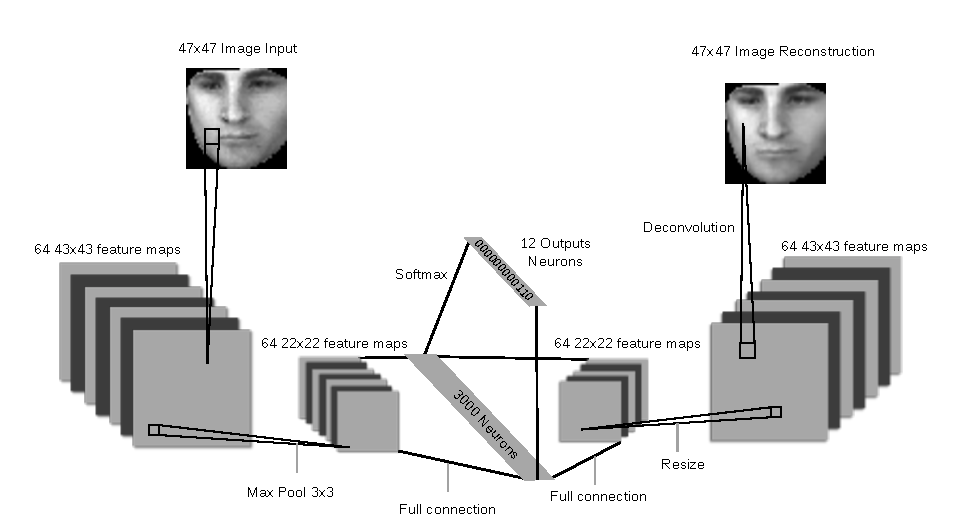
\includegraphics[width=\textwidth]{illustrations/aec_network.pdf}
     \captionof{figure}{General structure of the proposed network. Each rectangle
     represents many layers of neurons and the thin lines represent connections between layers.}
    \end{figure}

    Deep learning is emerging as a powerful tool in modelling a wide range of patterns
    in data, it has been applied to the problem of FAU a number of times and achieved
    good classification rates. One complication which arises when using Deep Neural
    Networks DNNs to classify AUs is that many frames are unlabelled (have neutral expressions)
    and hence the standard supervised DNN do not make good use of this information.
    This project aims to investigate how an autoencoder could be combined with the
    already established deep learning methods related to FAU in order to improve the performance
    of these techniques and better leverage unlabelled data. This unlabelled data may
    come from within the standard AU datasets or from larger databases of faces.
    The DISFA dataset is chosen for initial experiments.
  \section{Potential Applications}
  \section{Contributions}
  \section{Thesis Outline}

\chapter{Background}

\section{Databases for FAU estimation}
Relevant for this work is a awareness of datasets which exist and which may be useful
for experiments. Here is a list of some which should be used in order to allow
this project to be comparable to work in the literature:

\begin{itemize}
    \item The DISFA database \cite{disfa}, which contains 27 subjects whose spontaneous
          facial expressions were captured in controlled recording conditions.
    \item CK+ \cite{Lucey2010} containing 123 subjects recorded with faces in strictly front positions.
    \item FERA 2015 BP4D-Spontaneous Dataset \cite{Valstar}:
          containing 41 subjects and 34 AUs, the subjects were young adults who
          spontaneously generated emotional responses to stimulus tasks.
\end{itemize}

This is just a small selection, however is it representative of the types of
datasets available. Each frame of the videos has a label which describes which AUs are
present and their intensity. Hence two distinct problems can be tackled here, intensity
estimation and classification, this work follows the classification route however
intensity estimation should also be possible with a few minor modifications.

A key challenge with these datasets is that they often have very unbalanced and
sparse labels as shown in figure \ref{disfastats}. This calls for methods
to balance training samples with respect to this imbalance and is the
motivation for using some unsupervised learning techniques, in order to extract information
from the unlabelled data.

A further two datasets are the TFD and SEMAINE, these do not contain AUs but often crop up in the
literature:
\begin{itemize}
     \item TFD \cite{tfd} Toronto Face Dataset
     \item The SEMAINE \cite{semaine} corpus which contains recordings
           of people interacting with a Sensitive Artificial Listener (SAL) in controlled conditions.
\end{itemize}

\section{The DISFA dataset} \label{disfa_list}
The Denver Intensity of Spontaneous Facial Action Dataset (DISFA)
Of central interest to the project is the DISFA dataset \cite{disfa}, it is a set
of videos of people watching 9 short clips from youtube which try to span a range
of emotions such as emotions happiness, surprise, fear, disgust and sadness. Included
are 27 subjects with 12 AUs.

Each frame in each subject video has a label which says how much of each AU is present on
a scale of 0-5, the distribution of intensities is shown in table \ref{compau}.

A challenge of the DISFA dataset is that it has many frames which are unlabelled, this is demonstrated
per subject in figure \ref{disfastats}. Many of the subjects have over 40\% of their frames unlabelled
, one outlier has over 75\% unlabelled.

\begin{table}[h!]
\centering

\begin{tabular}{lllllll}
\hline
Intensity & 0      & 1     & 2     & 3     & 4    & 5    \\ \hline
AU1       & 112286 & 2272  & 1749  & 2809  & 1393 & 555  \\
AU2       & 99165  & 1720  & 934   & 3505  & 836  & 369  \\
AU4       & 106160 & 4661  & 7636  & 6586  & 4328 & 1383 \\
AU5       & 99015  & 1579  & 719   & 293   & 104  & 34   \\
AU6       & 106425 & 9157  & 5986  & 3599  & 601  & 141  \\
AU9       & 99458  & 1659  & 2035  & 3045  & 316  & 77   \\
AU12      & 99987  & 13943 & 6869  & 7233  & 2550 & 172  \\
AU15      & 108358 & 5180  & 1618  & 1017  & 47   & 0    \\
AU17      & 117824 & 6342  & 4184  & 2281  & 112  & 11   \\
AU20      & 121377 & 1591  & 1608  & 1305  & 28   & 0    \\
AU25      & 84721  & 9805  & 13935 & 15674 & 5580 & 1039 \\
AU26      & 105778 & 13443 & 7473  & 3529  & 314  & 217  \\ \hline
\end{tabular}
\caption{A comparison of the number of occurrences of each intensity for each AU in the DISFA dataset} \label{compau}
\end{table}


\begin{figure}[h!]
  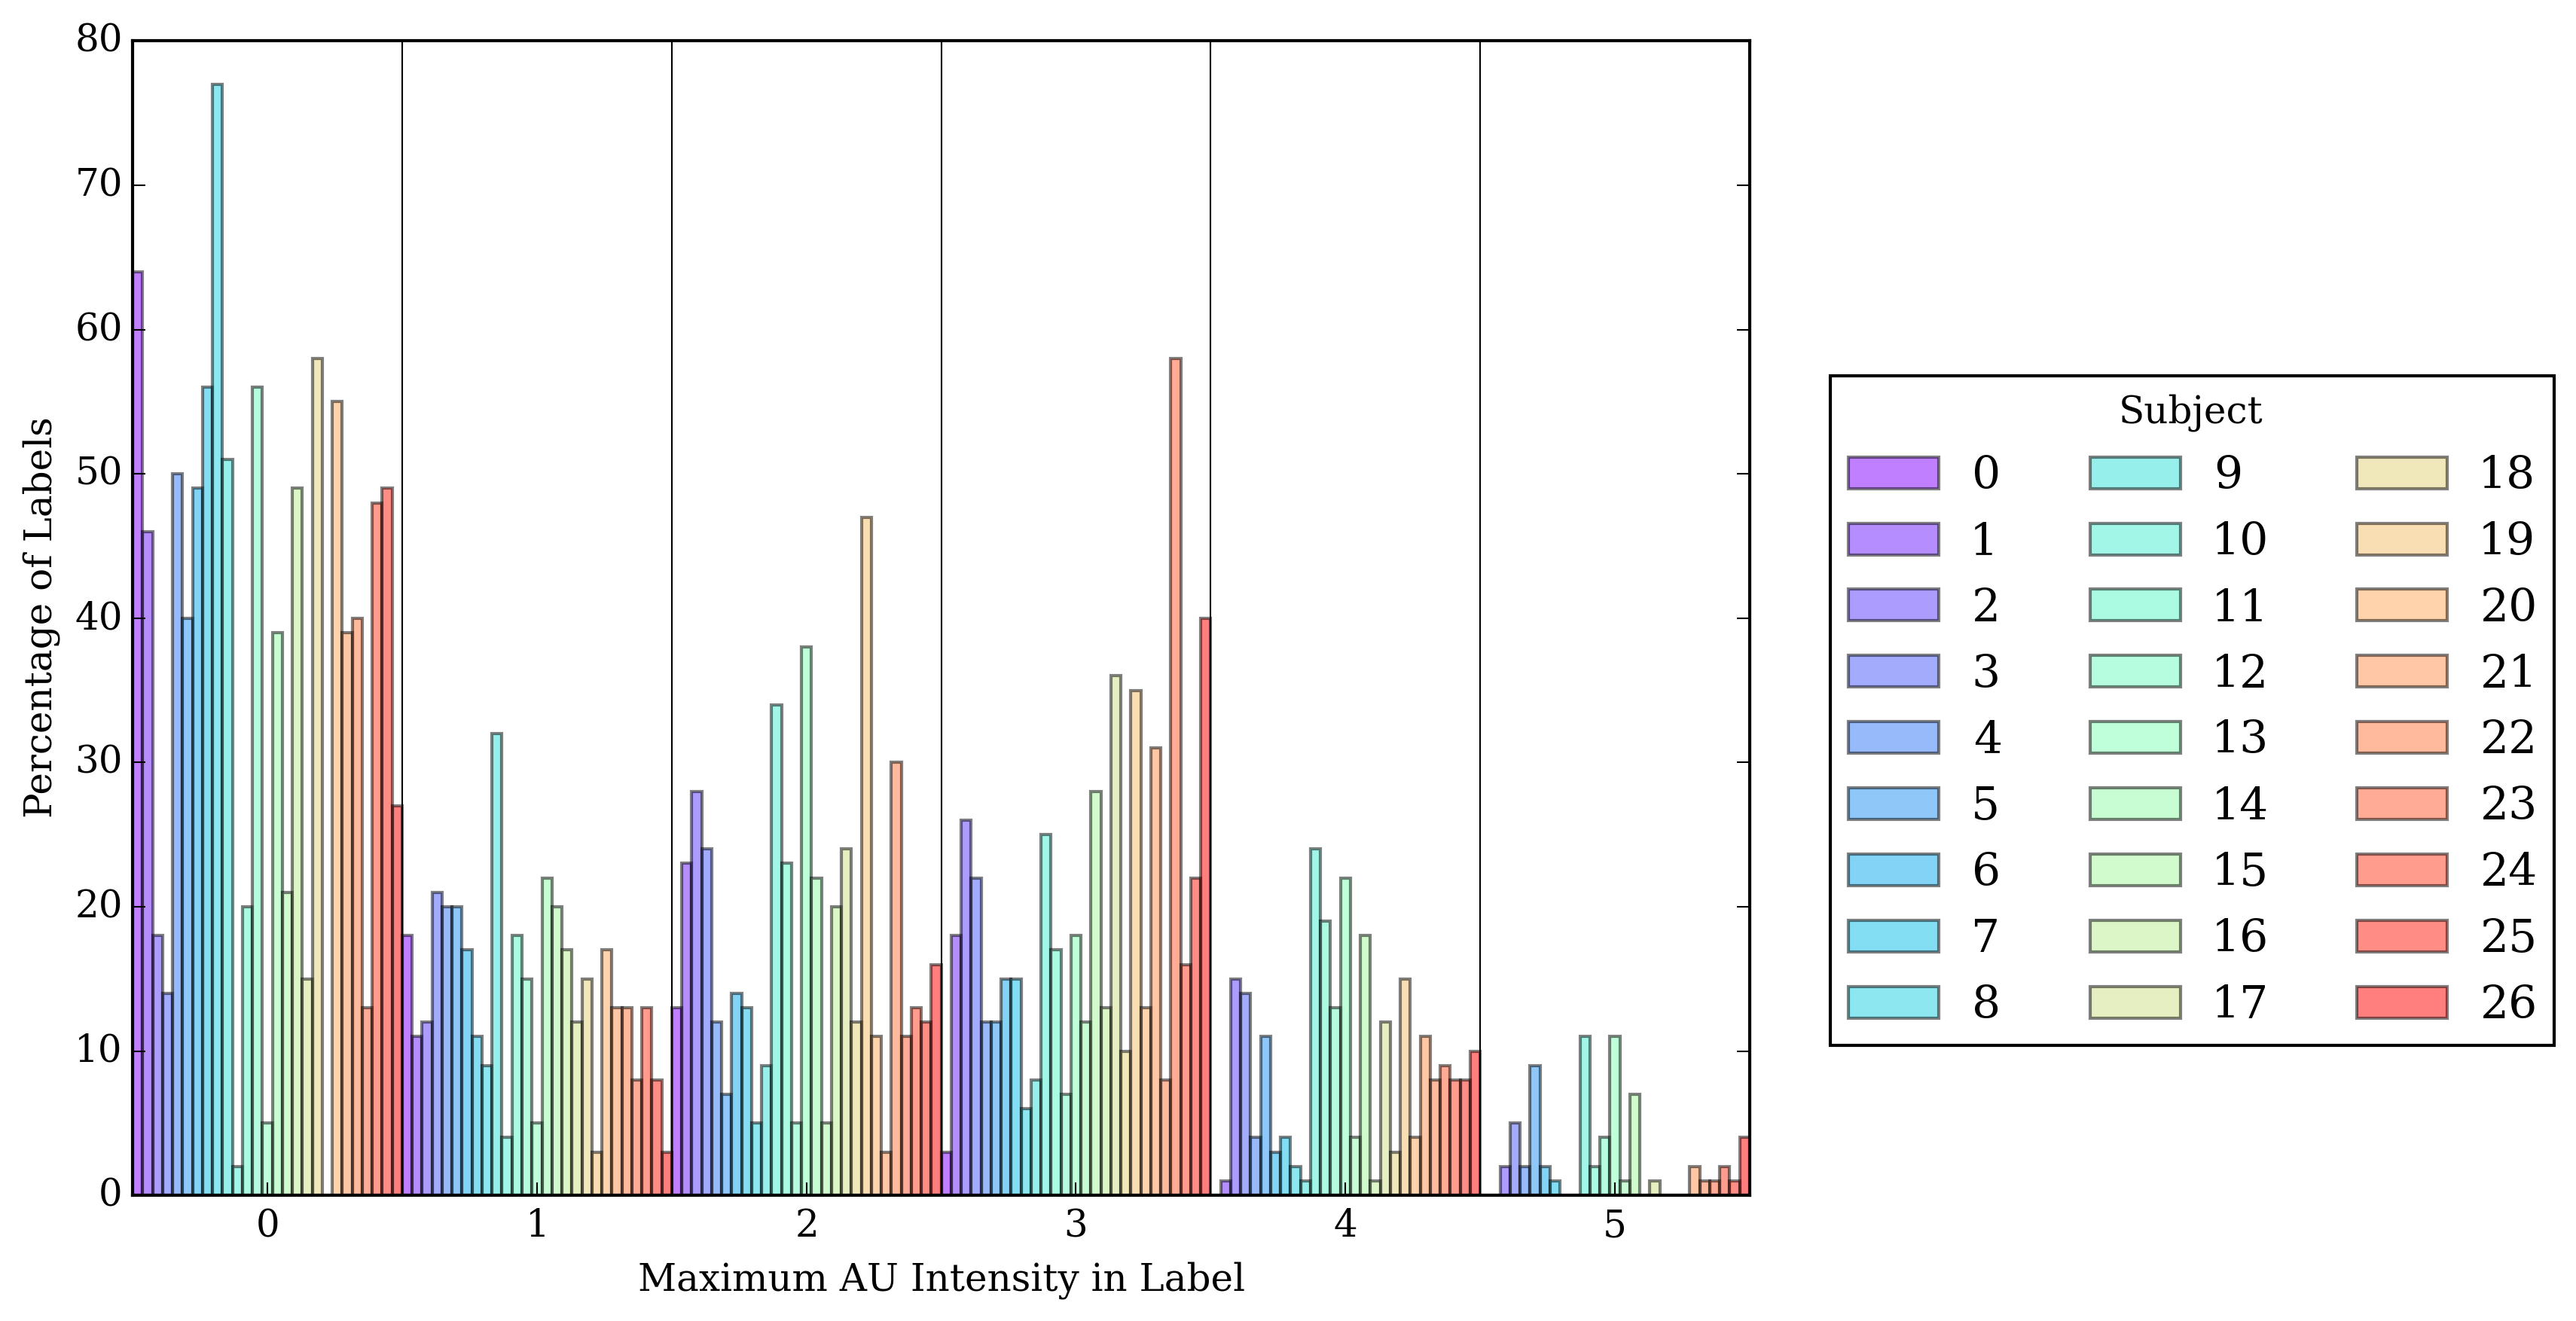
\includegraphics[width=\textwidth]{../graphs/maximum_label_intensity_disfa.pdf}
  \caption{DISFA dataset: This graph shows what the maximum value in each label is in the DISFA dataset per subject. This
  is done to illustrate the number of labels which contain very little information
  and pose an issue for a typical neural network structure.}\label{disfastats}
\end{figure}
\newpage

\section{Deep learning approaches to FAU detection}
It has been shown that deep neural networks containing convolutional, max pooling,
dropout and fully connected layers can effectively learn how to classify AUs in
a selection of datasets \cite{Gudi2015,Ghosh2015,dodeeplearn}. For theoretical information
about these networks see Chapter \ref{chapter:deep} These
works only include networks which ignore the temporal structure of the data,
other architectures do incorporate this \cite{emonet,Jaiswal2016}.
%
%
%
\subsection*{Comparison of networks in Table \ref{compnet}}
Network \cite{Ghosh2015} (Ghosh et al.) was trained on CK+, DISFA and BP4D datasets.
A key result of this paper was that they achieved good generalisation between datasets
with classifications accuracies between 60\% and 80\% for these generalisation experiments.
A feature particular to this network was that after the softmax layer, which assigns probabilities
to each AU it uses QDA (Quadratic Discriminant Analysis) \cite{precogbook} to
make predictions about whether AUs are present. A point of interest is also that
mean face normalisation is done per subject and then all for all subjects.

Network \cite{Gudi2015} (Amogh Gudi et al.) was trained on BP4D and SEMAINE
datasets achieving an average F1 score of 0.52 and 0.34 respectively. This paper
uses minimal preprocessing hence is a good example of how CNNs can learn features
with little feature engineering.

Network \cite{dodeeplearn} (Pooya Khorrami et al.) was trained on TFD and CK+,
this got average accuracies of 89.9\% and 98.3\% respectively in detecting emotions. This
is therefore not directly comparable, but they do explore connecting it with AUs.
An interesting point about this work is that they could stimulate activations in the convolutional
layers and directly see that the network had learned different facial actions demonstrating the
power of these networks.

Network \cite{Jaiswal2016} (Shashank Jaiswal et al.) was trained on SEMAINE and
BP4D achieving an overall weighted F1 score of 0.54. Which is on average higher
than network \cite{Gudi2015} as claimed in the paper. This paper includes a lot more
prior knowledge than the others, firstly it uses a BLSTM to incorporate temporal structure
and it defines multiple input streams from each facial region, allowing the convolutional
filters to become more specialised. This is the only paper where they say they use
two outputs for each AU so that the softmax creates a probability distribution for
each AU and not for all of them at once.

It should be noted that it is difficult to compare the performance between these
networks as they all use different evaluation scores as shown in table \ref{compscore}.

\begin{table}[h!]
\centering
{\footnotesize
\begin{tabular}{|lllllllll|}
\hline
Network                      & \multicolumn{2}{c}{Ghosh et. al\cite{Ghosh2015}}                         & \multicolumn{2}{c}{Gudi et. al.\cite{Gudi2015}}                            & \multicolumn{2}{c}{Khorrami et. al.\cite{dodeeplearn}}                          & \multicolumn{2}{c|}{Jaiswal et. al.\cite{Jaiswal2016}}   \\ \hline
\multicolumn{1}{|l|}{Element} & Type     & \multicolumn{1}{l|}{Dimensions}                    & Type     & \multicolumn{1}{l|}{Dimensions}                      & Type          & \multicolumn{1}{l|}{Dimensions}                  & Type      & Dimensions                     \\ \hline
\multicolumn{1}{|l|}{x}       &          & \multicolumn{1}{l|}{$40\times40\times1$}           &          & \multicolumn{1}{l|}{$48\times 48\times1$}            &               & \multicolumn{1}{l|}{$96\times96\times1$}         &           & $?\times?\times1$              \\ \hline
\multicolumn{1}{|l|}{$L_1$}   & conv 1   & \multicolumn{1}{l|}{$12\times 12\times1\times 70$} & conv 1   & \multicolumn{1}{l|}{$5\times 5\times1\times64$}      & conv 1        & \multicolumn{1}{l|}{$5\times5\times1\times64$}   & conv 1*   & $5\times5\times(2n+1)\times32$ \\
\multicolumn{1}{|l|}{$y_1$}   &          & \multicolumn{1}{l|}{$29\times29\times70$}          &          & \multicolumn{1}{l|}{$44\times44\times64$}            &               & \multicolumn{1}{l|}{$92\times92\times64$}        &           & $?\times?\times32$             \\ \hline
\multicolumn{1}{|l|}{$L_2$}   & max pool & \multicolumn{1}{l|}{$2\times 2$}                   & max pool & \multicolumn{1}{l|}{$3\times3$ (stride 2)}           & max pool      & \multicolumn{1}{l|}{$2\times2$}                  & max pool*  & $3\times3$                    \\
\multicolumn{1}{|l|}{$y_2$}   &          & \multicolumn{1}{l|}{$15\times15\times 70$}         &          & \multicolumn{1}{l|}{$22\times 22\times64$}           &               & \multicolumn{1}{l|}{$46\times46\times64$}        &           & $?\times?\times32$             \\ \hline
\multicolumn{1}{|l|}{$L_3$}   & conv 2   & \multicolumn{1}{l|}{$4\times 4\times70\times 10$}  & conv 2   & \multicolumn{1}{l|}{$5 \times 5 \times 64\times64$}  & conv 2        & \multicolumn{1}{l|}{$5\times5\times64\times128$} & conv 2    & $5\times5\times32\times64$     \\
\multicolumn{1}{|l|}{$y_3$}   &          & \multicolumn{1}{l|}{$12\times 12 \times 10$}       &          & \multicolumn{1}{l|}{$18 \times 18\times64$}          &               & \multicolumn{1}{l|}{$42\times42\times128$}       &           & $?\times?\times64$             \\ \hline
\multicolumn{1}{|l|}{$L_4$}   & max pool & \multicolumn{1}{l|}{$2\times 2$}                   & conv 3   & \multicolumn{1}{l|}{$4\times 4 \times64 \times 128$} & max pool      & \multicolumn{1}{l|}{$2\times2$}                  & conv 3    & $5\times5\times64\times64$     \\
\multicolumn{1}{|l|}{$y_4$}   &          & \multicolumn{1}{l|}{$6\times 6 \times 12$}         &          & \multicolumn{1}{l|}{$15\times15\times128$}           &               & \multicolumn{1}{l|}{$21\times21\times128$}       &           & $?\times?\times64$             \\ \hline
\multicolumn{1}{|l|}{$L_5$}   & fc       & \multicolumn{1}{l|}{$500$}                         & fc       & \multicolumn{1}{l|}{$3072$}                          & conv 3        & \multicolumn{1}{l|}{$5\times5\times1\times256$}  & conv 3    & $4\times4\times64\times128$    \\
\multicolumn{1}{|l|}{$y_5$}   &          & \multicolumn{1}{l|}{$500$}                         &          & \multicolumn{1}{l|}{$3072$}                          &               & \multicolumn{1}{l|}{$17\times17\times256$}       &           & $?\times?\times128$            \\ \hline
\multicolumn{1}{|l|}{$L_6$}   & fc       & \multicolumn{1}{l|}{$100$}                         & softmax  & \multicolumn{1}{l|}{$12$}                            & quadrant pool & \multicolumn{1}{l|}{}                            & fc        & $3072$                         \\
\multicolumn{1}{|l|}{$y_6$}   &          & \multicolumn{1}{l|}{$100$}                         &          & \multicolumn{1}{l|}{$12$}                            &               & \multicolumn{1}{l|}{$4\times4\times256$}         &           & $3072$                         \\ \hline
\multicolumn{1}{|l|}{$L_7$}   & softmax  & \multicolumn{1}{l|}{$12$}                          &          & \multicolumn{1}{l|}{}                                & fc            & \multicolumn{1}{l|}{$300$}                       & softmax   & $2N_{C}$                       \\
\multicolumn{1}{|l|}{$y_7$}   &          & \multicolumn{1}{l|}{$12$}                          &          & \multicolumn{1}{l|}{}                                &               & \multicolumn{1}{l|}{$300$}                       &           & $2N_{C}$                       \\ \hline
\multicolumn{1}{|l|}{$L_8$}   & QDA      & \multicolumn{1}{l|}{}                              &          & \multicolumn{1}{l|}{}                                & softmax       & \multicolumn{1}{l|}{$8$}                         & BLSTM     &                                \\
\multicolumn{1}{|l|}{$y_8$}   &          & \multicolumn{1}{l|}{}                              &          & \multicolumn{1}{l|}{}                                &               & \multicolumn{1}{l|}{$8$}                         &           &                                \\ \hline
\end{tabular}

\caption{A comparison of network architectures from the literature, all networks
use RELUs as their activation functions apart from in the final layer where it is
typical to use a softmax. $x$ denotes the input image, $L_i$ denotes the $i$th layer and $y_i$ denotes the output of the $i$th layer.
$N_{C}$ is the number of classes.
The question marks signify the dimensions of input images are variable as it depends on the input stream. fc is for fully connected and
conv is for convolutional layer. QDA is Quadratic Discriminant Analysis and BLSTM is for Bidirectional Long Short-Term Memory neural
networks.
\newline
*These layers are per input stream} \label{compnet}

}
\end{table}

\begin{table}[h!]
\centering

\begin{tabular}{lcccc}
\hline
Score    & \multicolumn{1}{l}{Ghosh et. al\cite{Ghosh2015}} & \multicolumn{1}{l}{Gudi et. al.\cite{Gudi2015}} & \multicolumn{1}{l}{Khorrami et. al.\cite{dodeeplearn}} & \multicolumn{1}{l}{Jaiswal et. al.\cite{Jaiswal2016}} \\ \hline
Accuracy & \checkmark                                       &                                                 & \checkmark                                             &                                             \\
F1       &                                                  & \checkmark                                      &                                                        & \checkmark                                  \\
AUC      &                                                  &                                                 &                                                        &                                             \\
2AFC     & \checkmark                                       & \checkmark                                      &                                                        &                                             \\ \hline
\end{tabular}
\caption{A comparison of which evaluation methods were used in the relevant papers.} \label{compscore}
\end{table}

\begin{table}[h!]
\centering

\begin{tabular}{lcccc}
\hline
Dataset    & \multicolumn{1}{l}{Ghosh et. al\cite{Ghosh2015}} & \multicolumn{1}{l}{Gudi et. al.\cite{Gudi2015}} & \multicolumn{1}{l}{Khorrami et. al.\cite{dodeeplearn}} & \multicolumn{1}{l}{Jaiswal et. al.\cite{Jaiswal2016}} \\ \hline
CK+      & \checkmark                            &                                      &                                         & \checkmark                              \\
DISFA    & \checkmark                            &                                      &                                         &                                         \\
SEMAINE* &                                       & \checkmark                           & \checkmark                              &                                         \\
BP4D*    & \checkmark                            & \checkmark                           & \checkmark                              &                                         \\
TFD      &                                       &                                      &                                         & \checkmark                              \\ \hline
\end{tabular}
\caption{A comparison of which datasets were used in the relevant papers.} \label{compdat}
\end{table}


%
%
%

\chapter{Implementation}
  \section{Deep Learning Framework}
    TensorFlow \cite{tensorflow} was chosen as the deep learning framework for this
    project. Many others such as Caffe, Neon, Theano, and Torch are popular\cite{Bahrampour2016}.
    The main advantages of TensorFlow are flexibility with running code on diverse
    hardware platforms and good support for visualisations
    of computation graphs. The other frameworks in fact are more efficient
    \footnote{TensorFlow even came last in one benchmark performed on the VGG-16 network, \url{https://github.com/aizvorski/vgg-benchmarks}}
    computationally due to their maturity\cite{Bahrampour2016}
    but this is not a major requirement in this project.

% TensorFlow is a very flexible framework, specially in
% employing homogeneous/heterogeneous devices for the
% various parts of the computational graph.

    Similar to most other frameworks TensorFlow uses python
    to define its computations and also has C++ interfaces for creating new operators.
    A TensorFlow application can run on either a GPU or CPU with no modification, this was
    a particularly nice feature as GPU resources are often scarce and if time is not an issue a CPU
    can perform the training and evaluation of a model in a reasonable time (1-5 hours). The GPU used in this project was a nVidia GTX Titan X.
  \section{Development Environment}
    The python scripts and notebooks produced were developed on two systems:
    \begin{itemize}
      \item     Ubuntu 14.04.4 LTS with TensorFlow 0.7.1, numpy 1.11.0. This setup typically utilised a GTX Titan X GPU with driver version 352.63, otherwise
                an Intel(R) Core(TM) i7-4790 CPU @ 3.60GHz or equivalent processor was used.
      \item     Ubuntu 15.10 with TensorFlow 0.9.0 and numpy 1.11.0. This setup had no GPU support but small models were still efficient to train on this set up
                despite the processor being a low power Intel® Core™ M-5Y10c CPU @ 0.80GHz.
    \end{itemize}
    Atom \footnote{Atom is a cross platform text editor - \url{https://atom.io/}}and PyCharm \footnote{PyCharm is a integrated development environment for the python language \url{https://www.jetbrains.com/pycharm/}} were used to edit all text and source files in the project.
    Atom due to its intuitive editing capabilities and extensive plugins. PyCharm because
    of its powerful refactoring capabilities and ability to discover syntax errors before
    a python script is run. PyCharm also nicely integrates with git \footnote{Git is an open source version control system,
    the git repository used for this project is found at \url{https://github.com/lotka/autofaces}}, which was used for version control.
    One use case of git was to identify, with a git commit id each experiment which was run, so that in the future
    anyone can see exactly which bits of python code at which time generated particular experimental results.
    SSH\footnote{Secure Shell (SSH) is a cryptographic network protocol used for interfacing with remote machines.} provided a convenient way to start jobs on machines remotely and tmux \footnote{Tmux is a terminal
    multiplexer which can keep SSH sessions active} was used to manage multiple jobs on multiple machines.

    For visualisation matplotlib was the staple tool used to plot graphs and images. iPython notebooks
    which can display many matplotlib graphs interspersed with text and code were heavily used to
    provide a simple direct way to analyse the output of a job. This quickly became the most convenient way to
    share and interpret experimental data. Tensorboard is part of TensorFlow which allows the monitoring of a
    model training session and some analysis, this was initially interesting but became too limited for the required purposes.
  \section{Reproducing results} \label{sec:GPU}
    Due to a slight limitation in TensorFlow\footnote{\url{https://github.com/tensorflow/tensorflow/issues/2732}}, results would often be non-deterministic by a small degree. This generally slowed
    the process of experimentation as some large computations had to be repeated in order to calculate a standard error in the metrics used.
  \section{Project Implementation}
    This project, in terms of software engineering, produced a piece of software which does the following:
    \begin{enumerate}
      \item Load and process a dataset.
      \item Define a model which is compatible with the loaded dataset
      \item Train the model on the dataset while storing training information
      \item Evaluate the model and automatically produce useful graphs and numerical information which might give insight into improving the model
      \item Store results in a format which allows them to be reproduced and understood in the future
    \end{enumerate}

    This was achieved with the code structure shown in section
    \ref{sec:codestruct}. This along with the code should be enough to explore
    the implementation, so a detailed description is omitted here, however there
    are a couple of key features which are relevant. Firstly, the code produces
    a folder containing as much information as possible related to the training
    and evaluation of a model. The model is saved and can be loaded back into
    memory for more training or evaluation. Another feature is that when a
    dataset is loaded and processed, it can be saved along with a hash of the
    parameters that created it, so that for future runs the preprocessing does
    not have to be run again.

    A set of notebooks facilitate the presentation of the evaluation results,
    examples of this are figures \ref{fig:compareresults} and
    \ref{fig:viewresult} which show parts of a typical session which includes
    the inspecting of graphs and tables. Currently only the DISFA dataset is
    supported in the code, but modification for more datasets would not pose
    much work.



    \subsection{Code Structure} \label{sec:codestruct}
      The following briefly describes what each part of the code base does and how it relates
      to other files.
      {\small
      \begin{itemize}
        \item   {\bf src/}
                \begin{sloppypar} \textit{All python files that are responsible for generating a model and it's evaluation data}\end{sloppypar}
                \begin{itemize}
                  \item {\bf includes/ }
                  \begin{sloppypar} \textit{Third party libraries.}\end{sloppypar}
                  \item {\bf config/ }
                  \begin{sloppypar} \textit{Configuration files which can be loaded into main.py}\end{sloppypar}
                  \item {\bf test/ }
                  \begin{sloppypar} \textit{Various python files for testing functionality.}\end{sloppypar}
                  \item {\bf old/ }
                  \begin{sloppypar} \textit{Old python files from early stages of the project}\end{sloppypar}
                  \item {\bf replay.py }
                  \begin{sloppypar} \textit{Opens an existing model and displays some statistics about the data that was used}\end{sloppypar}
                  \item {\bf tidy.py }
                  \begin{sloppypar} \textit{Deletes incomplete experiments.}\end{sloppypar}
                  \item {\bf results.py }
                  \begin{sloppypar} \textit{Used by viewResult.ipynb and compareResults.ipynb to open an existing experiment, plot it's results and load it's results.}\end{sloppypar}
                  \item {\bf main.py }
                  \begin{sloppypar} \textit{Trains and evaluates models, calling all python scripts listed below. It requires a configuration file, a device and a flag which chooses whether to train multiple models while varying parameters or to just train one model.}\end{sloppypar}
                  \item {\bf alpha.py }
                  \begin{sloppypar} \textit{Defines the balance functions shown in section \ref{sec:autoalpha} }\end{sloppypar}
                  \item {\bf disfa.py }
                  \begin{sloppypar} \textit{Defines a class which on construction loads and preprocesses DISFA data}\end{sloppypar}
                  \item {\bf expman.py }
                  \begin{sloppypar} \textit{Manages configuration files and data storage directories.}\end{sloppypar}
                  \item {\bf helper.py }
                  \begin{sloppypar} \textit{Miscellaneous helper functions used throughout}\end{sloppypar}
                  \item {\bf metric.py }
                  \begin{sloppypar} \textit{Implements the techniques described in section \ref{sec:eval} }\end{sloppypar}
                  \item {\bf model.py }
                  \begin{sloppypar} \textit{Defines a TensorFlow graph describing the neural networks used in this project.}\end{sloppypar}
                  \item {\bf test\_set\_analysis.py }
                  \begin{sloppypar} \textit{Runs the test set through a fully trained model and saves results. Is used in main.py and can be used on its own.}\end{sloppypar}
                \end{itemize}
        \item   {\bf notebooks/ }
                \begin{sloppypar} \textit{iPython notebooks, generally used for visualisation of results and testing parts of the pipeline.}\end{sloppypar}
                \begin{itemize}
                  \item {\bf alpha\_function\_test.ipynb }
                  \begin{sloppypar} \textit{Plots functions in src/alpha.py}\end{sloppypar}
                  \item {\bf compareResults.ipynb }
                  \begin{sloppypar} \textit{Compares many experiment runs, used to generate the tables in section \ref{sec:model}}\end{sloppypar}
                    \begin{figure}[!h]
                    \centering
                    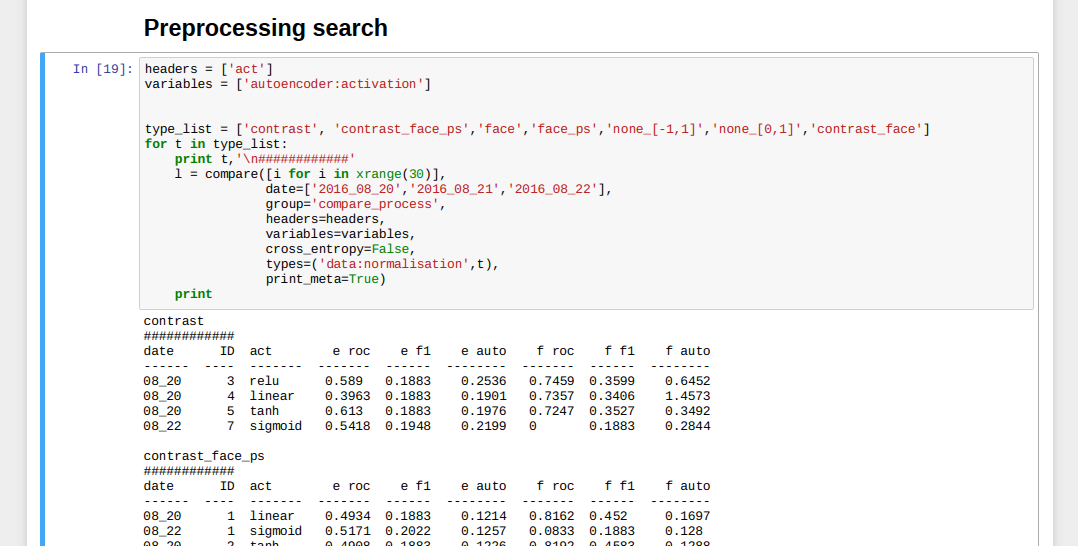
\includegraphics[width =0.8\hsize]{figures/notebook2.png}
                    \caption{{\bf compareResults.ipynb: }An example of an ipython script which compares the results of a selection of experiments,
                    this was used heavily to quickly produce the tables in the Results section.}
                    \label{fig:compareresults}
                    \end{figure}
                  \item {\bf viewResult.ipynb }
                  \begin{sloppypar} \textit{Visualises one run of main.py with many graphs and numerical results.}\end{sloppypar}
                    \begin{figure}[!h]
                    \centering
                    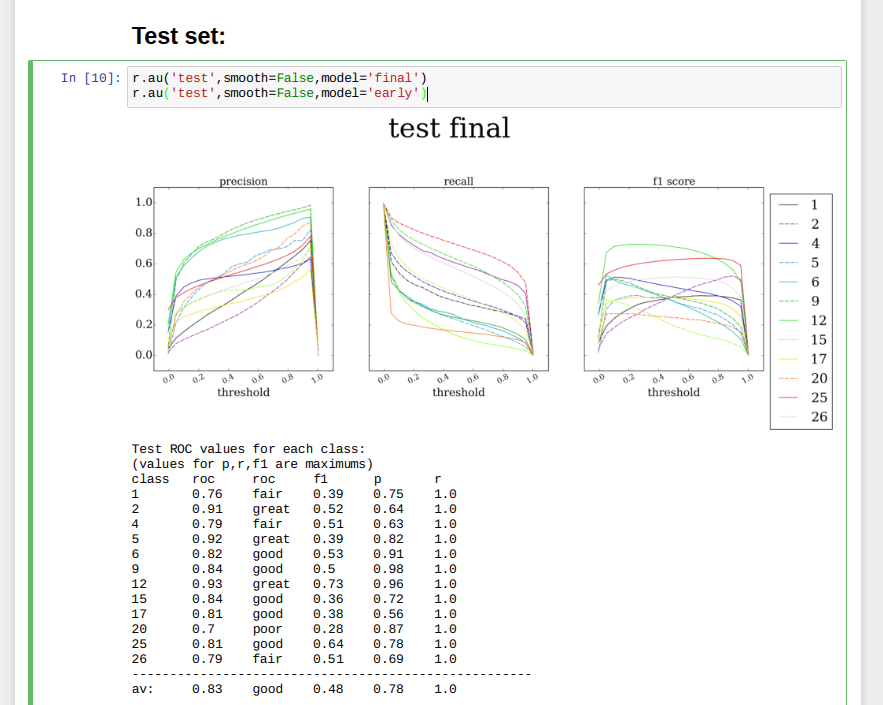
\includegraphics[width =0.8\hsize]{figures/notebook1.png}
                    \caption{{\bf viewResult.ipynb: } A small part of the notebook showing graphs related to F1, Precision and ROC for one experiment.}
                    \label{fig:viewresult}
                    \end{figure}
                  \item {\bf DisfaTest.ipynb }
                  \begin{sloppypar} \textit{Generates the graphs shown in section \ref{sec:methods}, this serves the purpose of
                    testing the preprocessing methods.}\end{sloppypar}
                \end{itemize}

      \end{itemize}
      }

\chapter{Data Preprocessing}
  \section{Introduction}
    It is typical to apply some sort of preprocessing operations to any data fed into
    a neural network. Although in theory a neural network can learn very complex
    non-linear transformations, it is often the case that learning this at the same
    time as learning other abilities is unrealistic. Preprocessing methods can
    also embed information about the dataset into each frame which the network is
    unlikely to learn as it works on a per example basis (this is a motivation for
    recurrent networks).
     Therefore it is vital to try
    different pre-processing methods on the data.
    It is also vital to try a range of methods
    because only a few
    might allow the autoencoder and classifier structures to cooperate with each other.
    This section describes some preprocessing methods which are to be
    tested in section \ref{sec:psearch}.

    % You should mention how: by a piece-wise
    % affine warp of the triangulated landmarks to a canonical shape.
    % And why: so that the facial regions within different
    % frames are aligned with each other, so that the network
    % does not need to account for spatial variations.

    The DISFA dataset as described in section \ref{disfa_list} has frames of size $ 1024 \times 764 $
    but using previous work of Sebastian Kaltwang\cite{Kaltwang2015} faces are
    centred and normalised by a piece-wise affine warp of the triangulated
    landmarks to a canonical shape to give an image of size $118 \times 128$
    with pixels being integers between
    0 and 255. An illustration is shown in figure \ref{fig:sebproc}.
    This is done in order to align face images with each other so that
    there is no need for the model to account for spatial variations.

    \begin{figure}[!h] \centering
    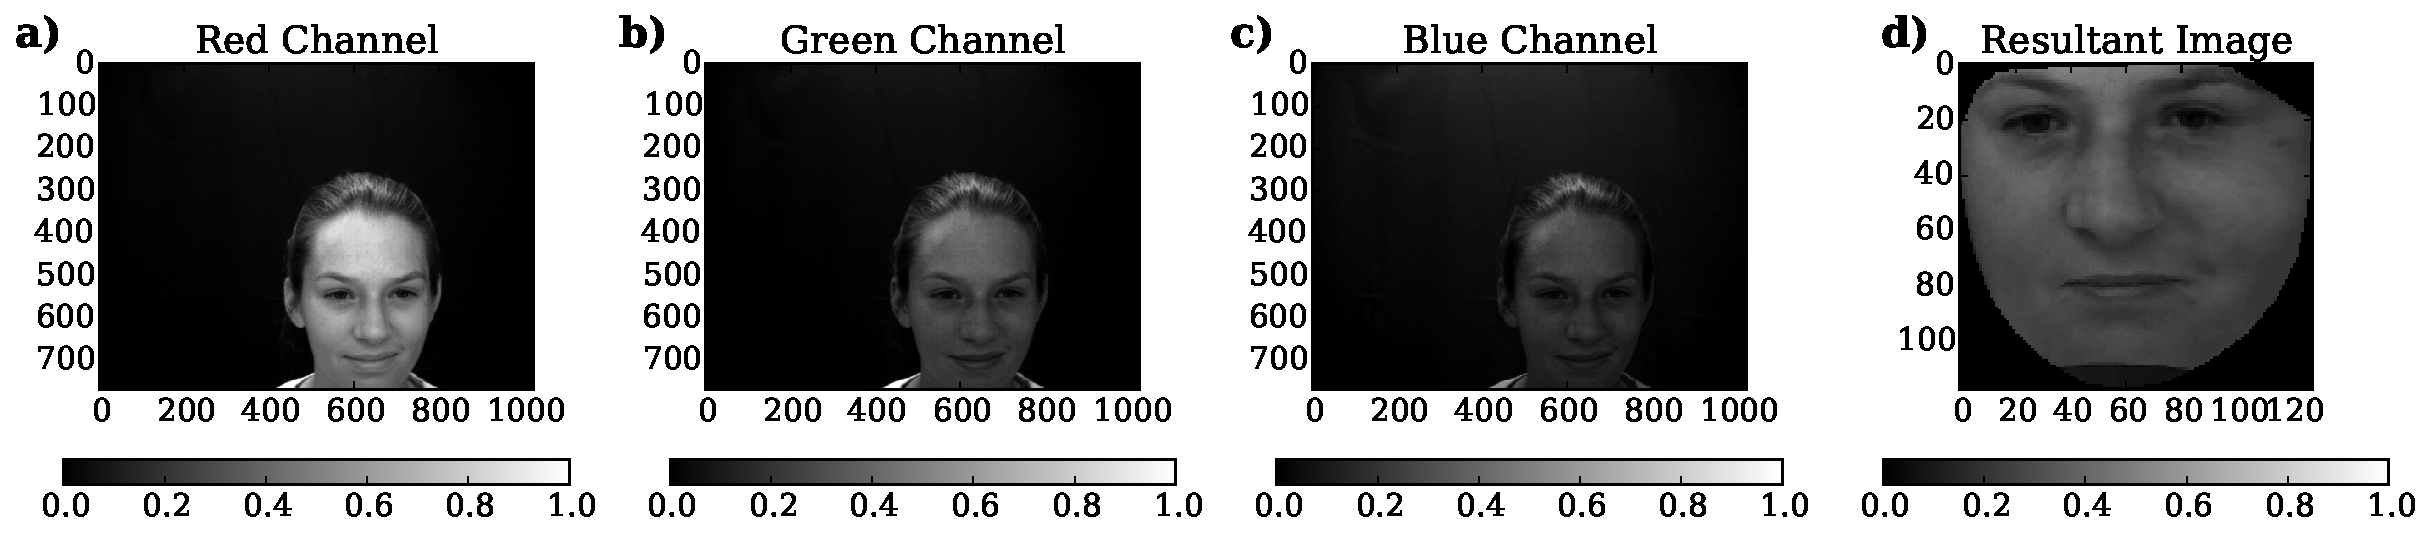
\includegraphics[width =\hsize]{figures/seb_preproc.pdf}
    \caption{ {\bf a) b) c)} An example of the original $764 \times 1024$ image with
    the 3 RGB channels displayed separately. {\bf d)} the resultant image
    $118 \times 128$ after face registration.} \label{fig:sebproc} \end{figure}


    This section first discusses the initial treatment of the labels.
    Then three different methods of normalising and scaling
    the dataset are described, these can be combined to create further methods. In order to illustrate
    the effect of such operations figures such as figure \ref{fig:faces_none} are used which
    show an example face and some statistical faces. The ideal method might
    have minimum and maximum faces which express high degrees of facial expression, so that
    high pixel values can easily be correlated to various AUs in the classifier. Another motivation
    for trying this many methods is to improve the chances of finding an input format which works will with both an
    autoencoder and classifier.

    \section{Methods For Labels}

      Labels are defined as a matrix:
      \begin{equation}
        {\bf y} \in \{0,1,2,3,4,5\}^{N\times F}
      \end{equation}

      Where $F$ is the number of AUs and $N$ is the number of labelled images
      in the dataset.

      Five is the highest intensity for an AU and zero is the absence of that
      AU. Typically a neural network outputs values between zero and one so
      these values are divided by five to make them compatible. For an intensity
      estimation problem that is all that is required, however for
      classification the AU labels need to be binary so a threshold is chosen at
      which an AU is considered present. Finally in the case of the Binary
      Softmax described in section \ref{sec:binsoft} the label vector needs to
      be expanded to also contain the negative case, hence doubling its size.

  \section{Methods For Images} \label{sec:methods}

    \begin{figure}[!h] \centering
    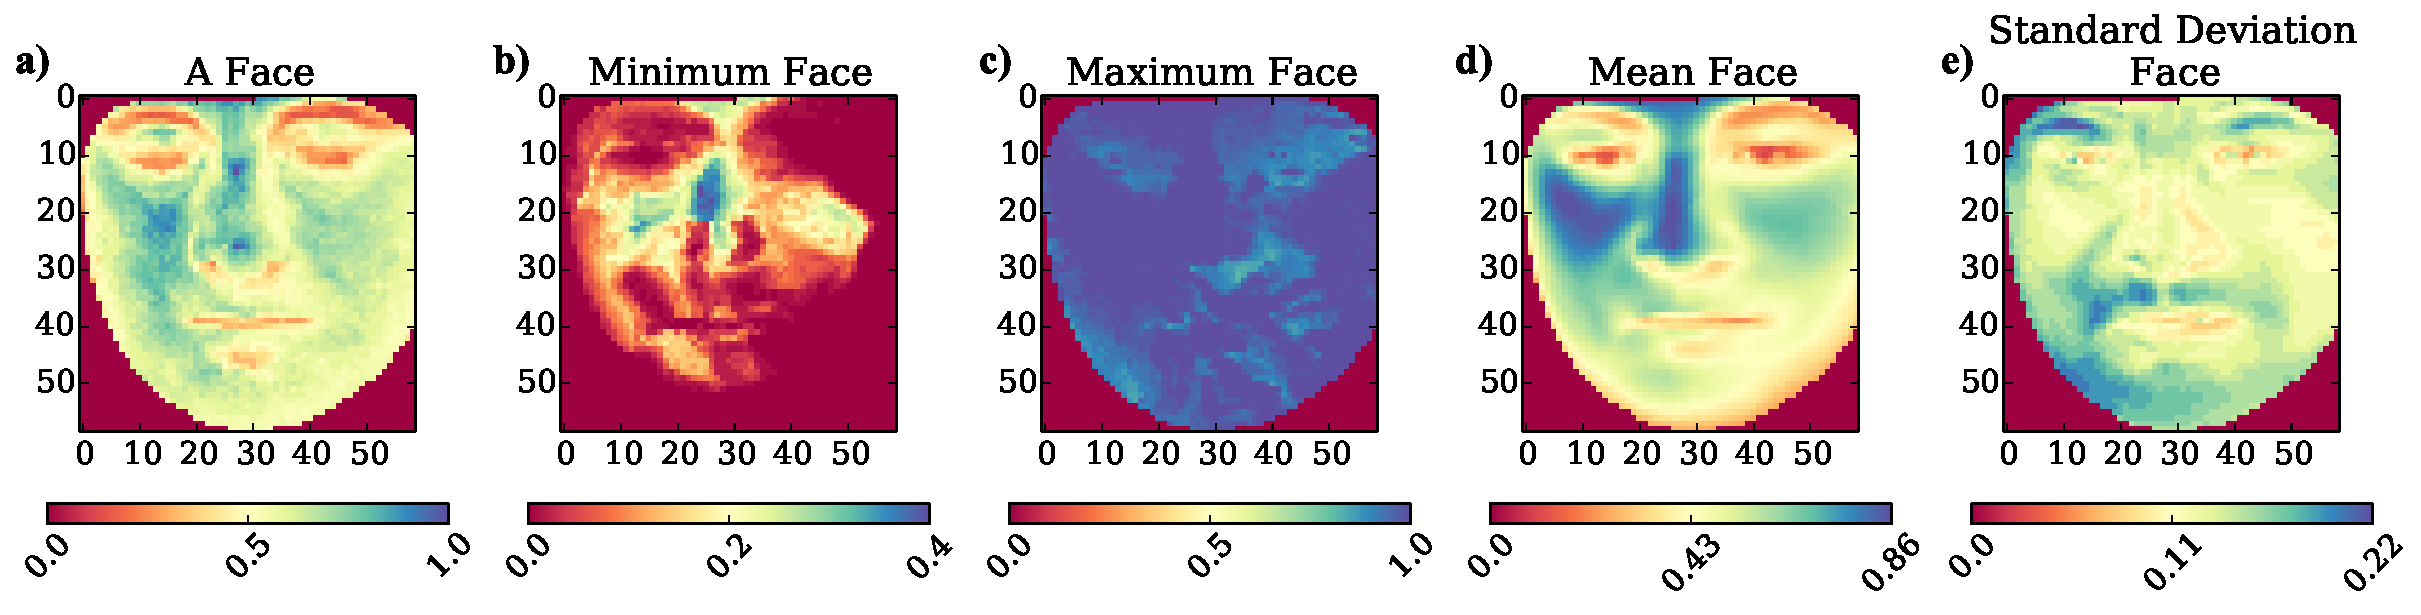
\includegraphics[width =\hsize]{figures/faces.pdf}
    \caption{The DISFA dataset with no preprocessing, it shows
    the images at the last stage of figure \ref{fig:sebproc}.
    Plots {\bf a)}, {\bf b)}, {\bf c)}, {\bf d)} and {\bf e)}
    correspond to a sample face, the minimum, the maximum,
    the mean and the standard deviation values of each pixel across
    the whole dataset respectively. The images were downscaled by a factor of 0.8 before being processed.}
    \label{fig:faces_none} \end{figure}

    The preprocessing methods assume that a dataset of a number of subjects
    is described as a matrix of the form:
    \begin{equation}
    {\bf x} \in \mathbb{R}^{N\times X \times Y},\quad {\bf y} \in \mathbb{N}^{N\times F}
    \end{equation}
    Where $\mathbf{x}$ contains the images, $\mathbf{y}$ contains the labels,
    $N$ is the number of images, $X$ is the width of the image, $Y$ is the height of the
    image and $F$ is the number of AUs labelled. Furthermore in some cases an extra dimension
    for the subject may be added:
    \begin{equation}
    {\bf x} \in \mathbb{R}^{S\times N\times X \times Y},\quad {\bf y} \in \mathbb{N}^{S\times N\times F}
    \end{equation}
    Some subjects may have a slightly different number of frames and this is reflected
    in the implementation but not in this section.

    Each preprocessing method will be denoted by a function ${\bf P}$ defined as follows:
    \begin{equation}
      {\bf P}({\bf x},i) = {\bf x'}_i
    \end{equation}
    For the per subject case:
    \begin{equation}
      {\bf P}({\bf x},i,s) = {\bf x'}_{si}
    \end{equation}
    Where $i$ indexes frames so has $0 \leq i < N$, where $N$ might be the number of frames
    in the whole dataset or just for a subject.

    This notation aims to express the fact that each image in the resultant dataset
    may use information from all other frames, as it is generated by a function of the dataset
    and it's own index $i$.

    %
    %
    %
    %
    %
    \subsection{Contrast Normalisation}
      \begin{figure}[!h]
      \centering
      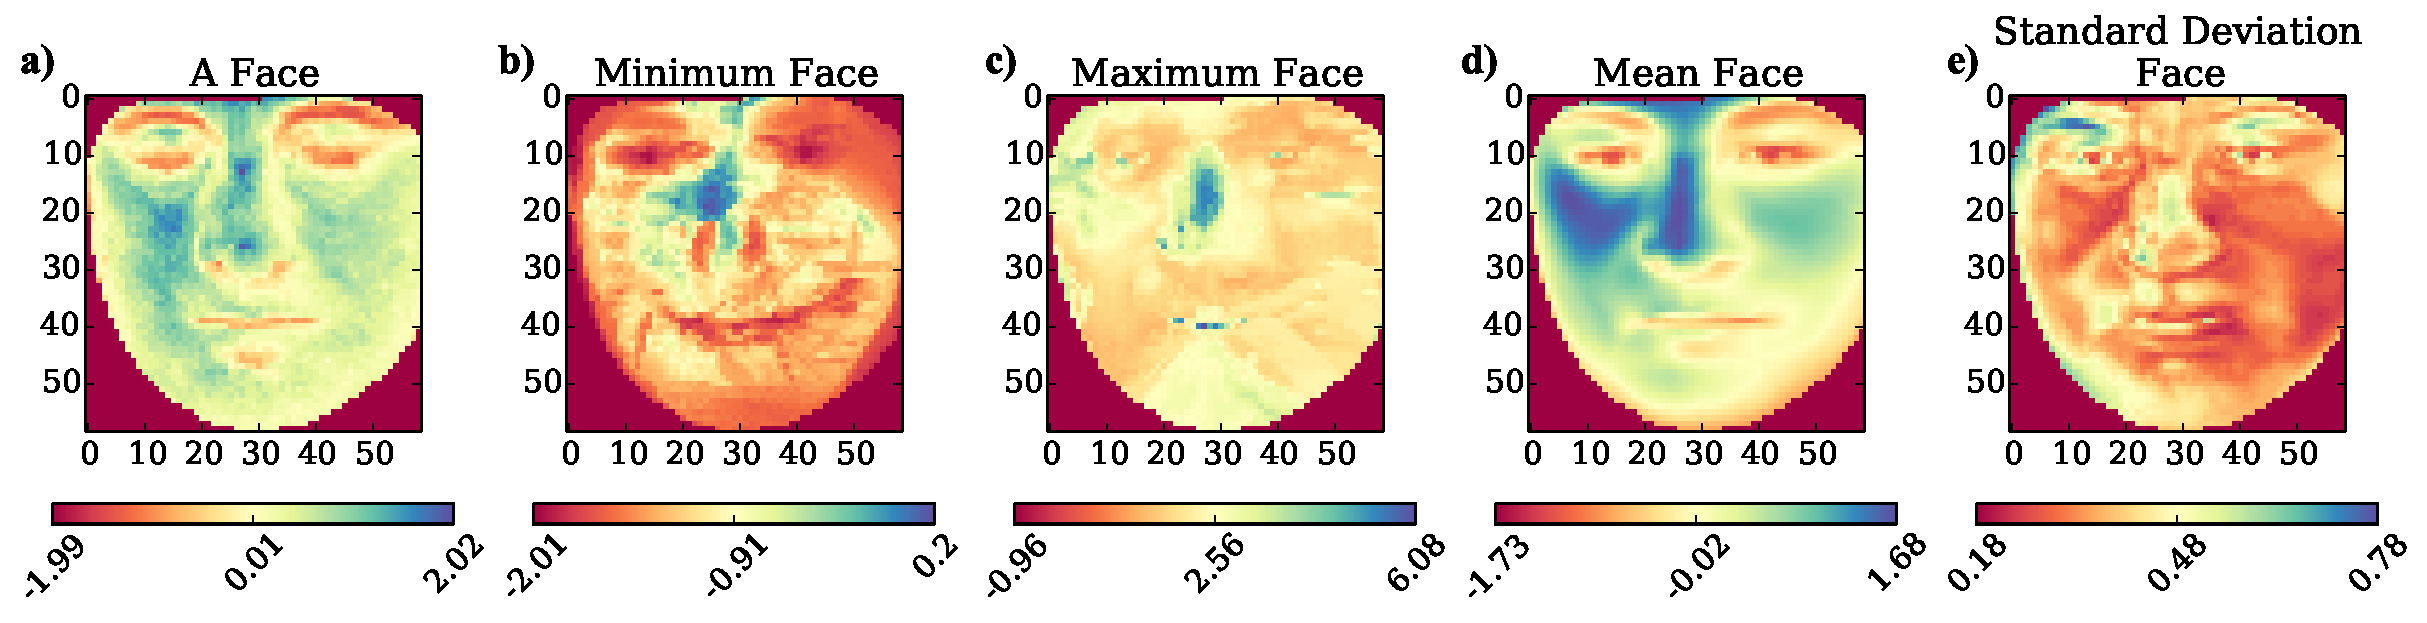
\includegraphics[width =\hsize]{figures/faces_contrast.pdf}
      \caption{The DISFA dataset with {\bf contrast normalisation}.
      Plots {\bf a)}, {\bf b)}, {\bf c)}, {\bf d)} and {\bf e)}
      correspond to a sample face, the minimum, the maximum,
      the mean and the standard deviation values of each pixel across
      the whole dataset. The images were downscaled by a factor of 0.8 before being processed.}
      \label{fig:fsdfhdfh}
      \end{figure}

      For each image find the mean pixel value and standard deviation and then subtract the mean
      and divide by the standard deviation. This standardises the amount of contrast in each image.
      \begin{equation}
         P({\bf x},i)= ({\bf x}_{i} - \mu({\bf x}_{i}))/\sigma ({\bf x}_{i}) = {\bf x}_{i}'
         \label{eq:con}
      \end{equation}
      Where $\mu$ and $\sigma$ gives the mean and standard deviation value of a matrix respectively.
      Equation \ref{eq:con} shows this, a disadvantage of this normalisation is that it
      has no regard of facial structures.

    %
    %
    %
    %
    %
    \subsection{Mean Face Normalisation} \label{sec:meanface}
      Here the mean face and standard deviation face is subtracted and divided away from the
      image, these faces might be per subject or per dataset, as shown:
      \begin{equation}
        P({\bf x},i) =  ({\bf x}_{i} - {\boldsymbol \mu}_0( {\bf x}))/{\boldsymbol \sigma}_0({\bf x}_{i})  = {\bf x}_{i}'
      \end{equation}
      \begin{equation}
        P_s({\bf x},s,i) = ({\bf x}_{si} - {\boldsymbol \mu}_{0}( {\bf x}_s))/{\boldsymbol \sigma}_{0}( {\bf x}_s))  = {\bf x}_{si}'
      \end{equation}
      Where ${\boldsymbol \mu}_{i,j..}$ denotes the mean over the axes $i,j..$ and
      similarly for ${\boldsymbol \sigma} $ the standard deviation.
      The point of this normalisation is to enhance the intensity of any pixels which
      are unusual, these pixels should hold most information about potential facial expressions.
      \begin{figure}[!h] \centering
      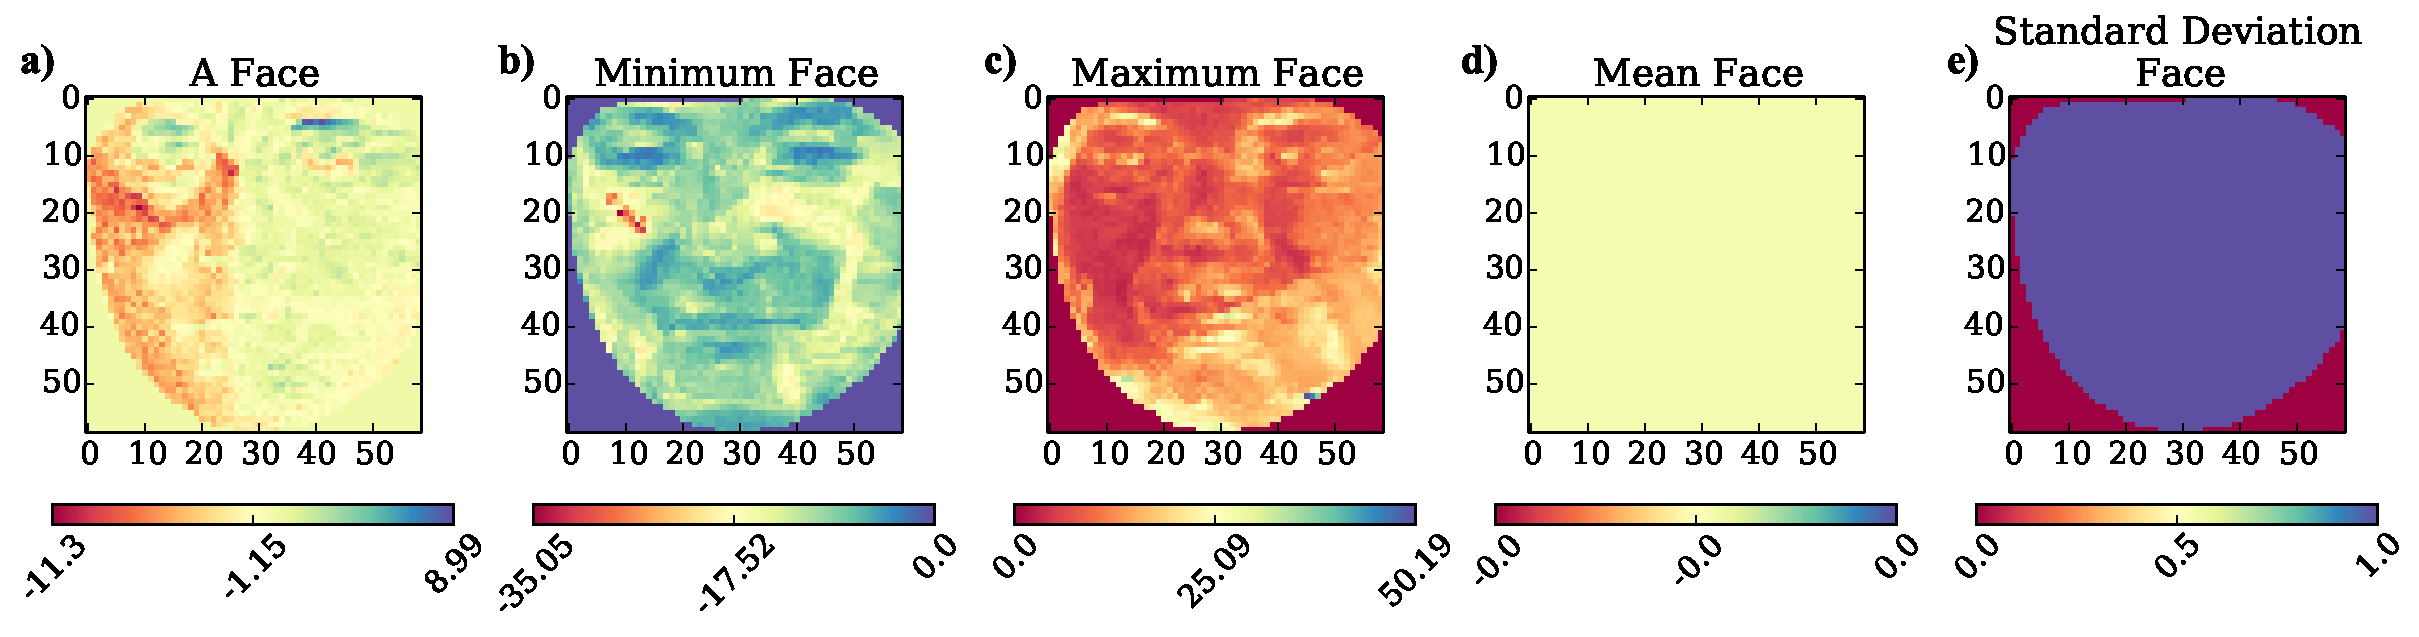
\includegraphics[width =\hsize]{figures/faces_per_subject_face.pdf}
      \caption{The DISFA dataset with {\bf per subject mean face normalisation}.
      Plots {\bf a)}, {\bf b)}, {\bf c)}, {\bf d)} and {\bf e)}
      correspond to a sample face, the minimum, the maximum,
      the mean and the standard deviation values of each pixel across
      the whole dataset. The images were downscaled by a factor of 0.8 before being processed.}
      \label{fig:}
      \end{figure}

    %
    %
    %
    %
    %
    \subsection{Range Scaling}
      This normalisation gets the data between the range of -1 and 1.
      \begin{equation}
        {\boldsymbol r}({\bf x})_{axis} = {\boldsymbol \min}_{axis}({\bf x}) - {\boldsymbol \min}_{axis}({\bf x})
      \end{equation}
      \begin{equation}
         P({\bf x},i) =
         \frac{{\bf x}_{i} - \frac{1}{2}\left ( {\boldsymbol \min}_0({\bf x}) + {\boldsymbol \min}_0({\bf x}) \right ) }{\frac{1}{2}{\boldsymbol r}_0({\bf x})}
         = {\bf x}_{i}'
      \end{equation}
      For the per subject case:
      \begin{equation}
         P_s({\bf x},i,s) =
         \frac{{\bf x}_{si} - {\boldsymbol \min}_0({\bf x}_s) - \frac{1}{2}{\boldsymbol r}_0({\bf x}_s) }{\frac{1}{2}{\boldsymbol r}_0({\bf x}_s)}
         = {\bf x}_{si}'
      \end{equation}
      \begin{figure}[!h] \centering
      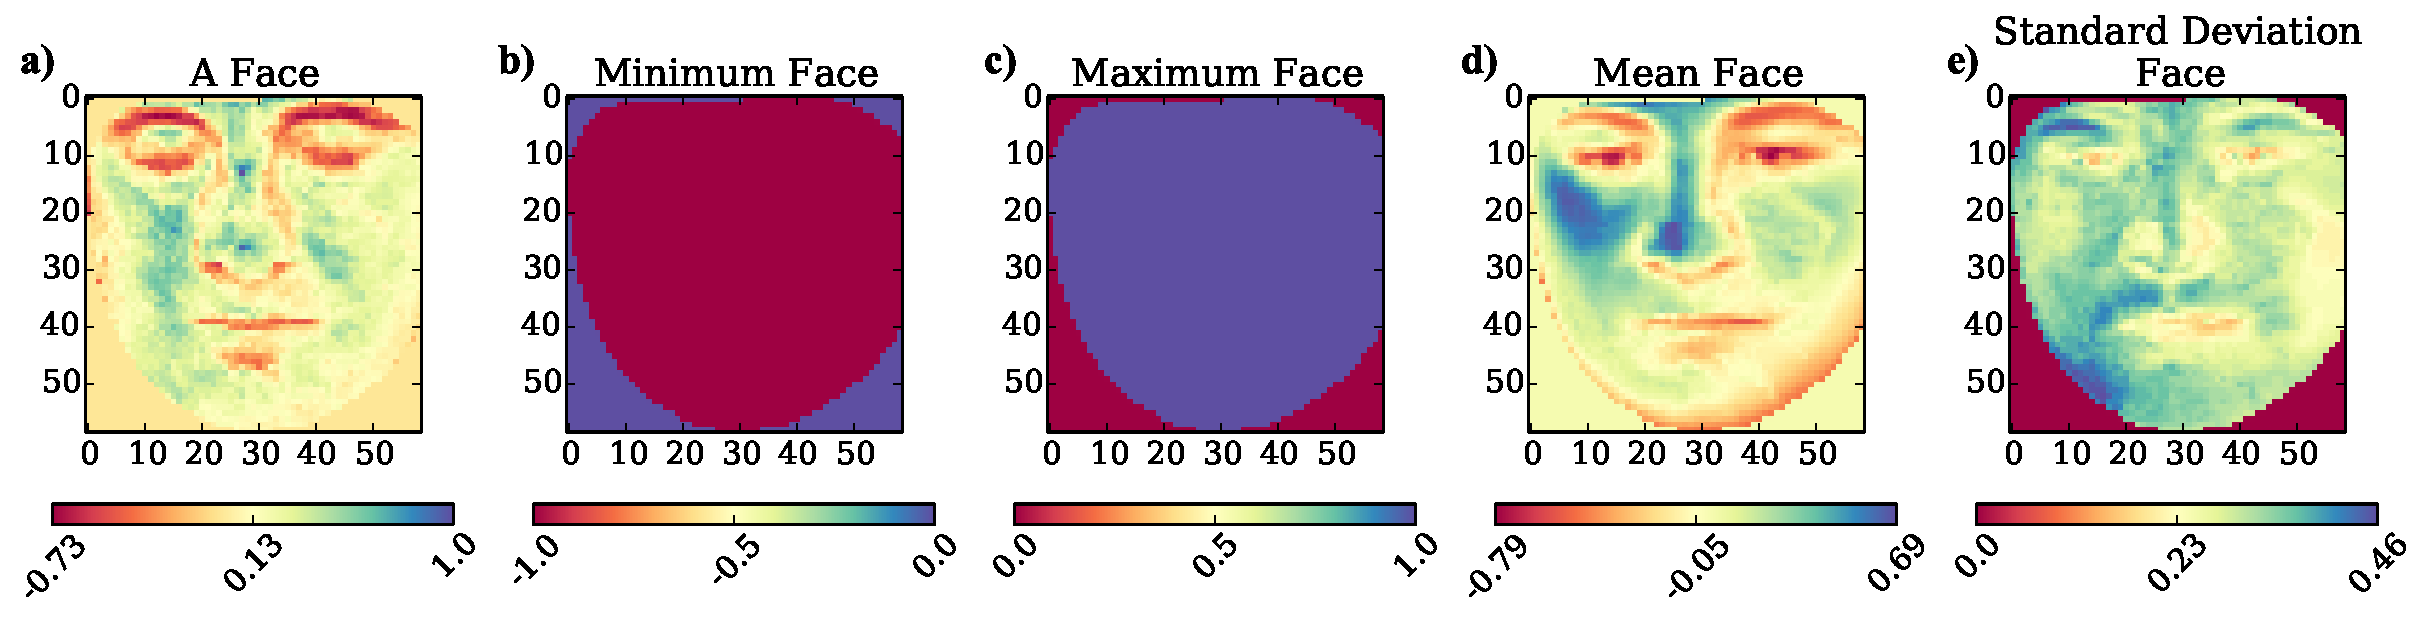
\includegraphics[width =\hsize]{figures/faces_range.pdf}
      \caption{The DISFA dataset with {\bf range scaling between -1 and 1}.
      Plots {\bf a)}, {\bf b)}, {\bf c)}, {\bf d)} and {\bf e)}
      correspond to a sample face, the minimum, the maximum,
      the mean and the standard deviation values of each pixel across
      the whole dataset. The images were downscaled by a factor of 0.8 before being processed.}
      \label{fig:simple} \end{figure}

    %
    %
    %
    %
    %
    \subsection{Combining methods}
      Some methods can be combined, figures \ref{fig:faces_contrast_face} and \ref{fig:faces_per_subject_contrast_face}
      shows the result of combining the mean face subtraction and then the
      contrast normalisation (in the per subject and whole set cases respectively). It is clear the effect is to
      reduce the range of the data, which may be useful for the classifier, however parts of the image
      which were all zero are now not which may result in lower performance.

      \begin{figure}[!h] \centering
      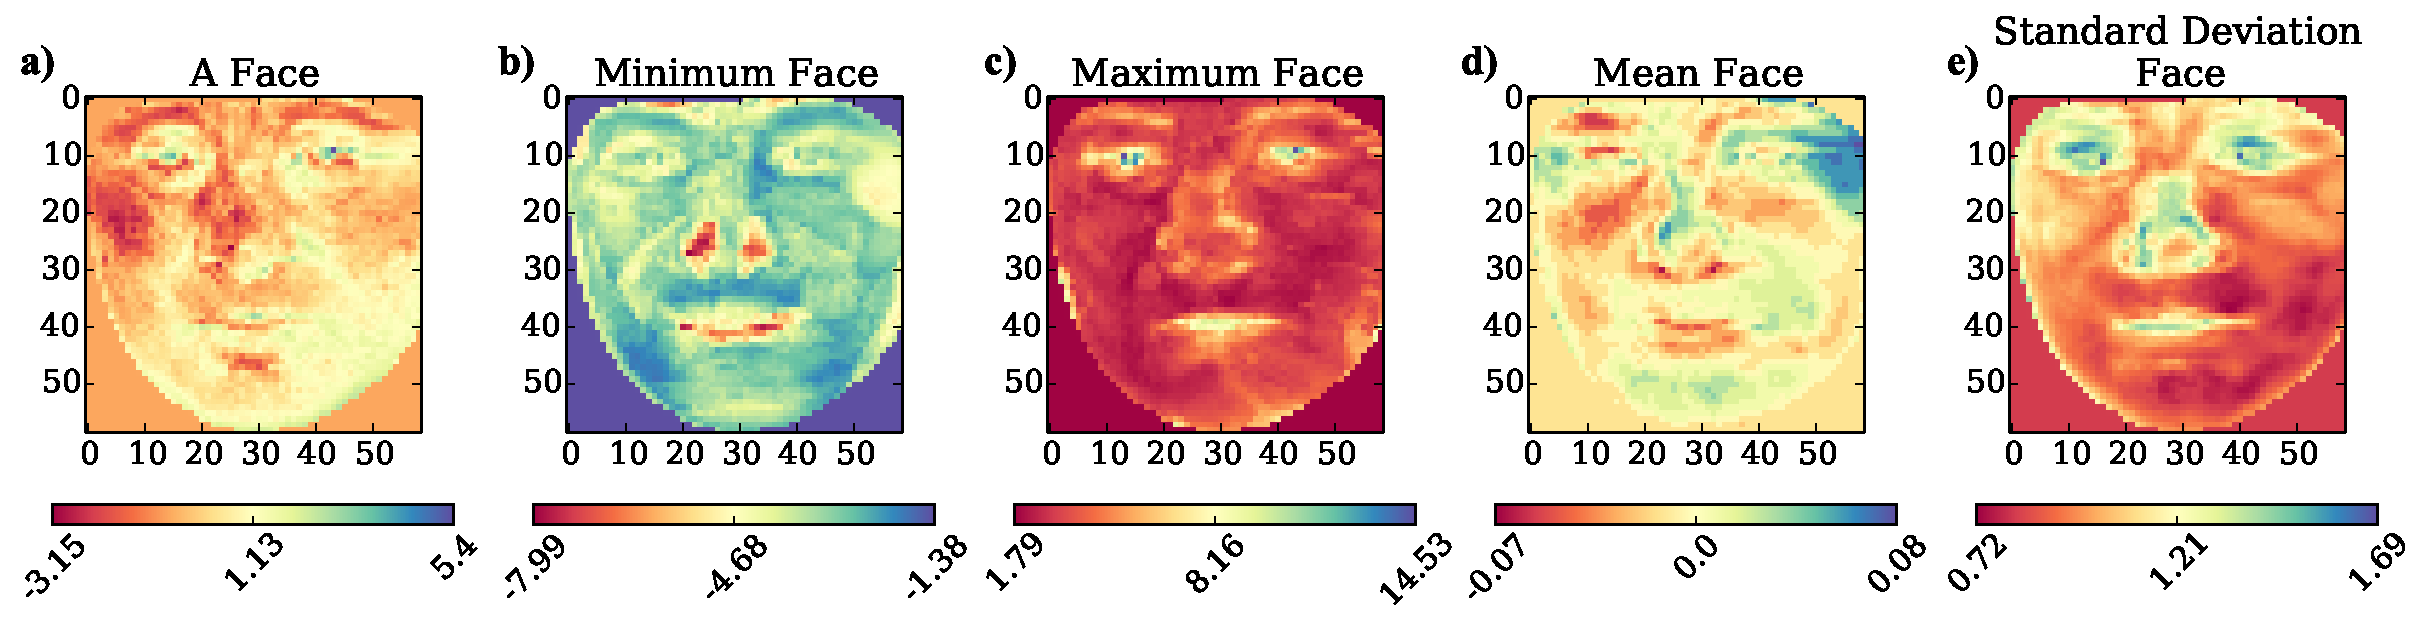
\includegraphics[width =\hsize]{figures/faces_contrast_face.pdf}
      \caption{The DISFA dataset with {\bf mean face normalisation and then contrast normalisation} applied.
      Plots {\bf a)}, {\bf b)}, {\bf c)}, {\bf d)} and {\bf e)}
      correspond to a sample face, the minimum, the maximum,
      the mean and the standard deviation values of each pixel across
      the whole dataset. The images were downscaled by a factor of 0.8 before being processed.}
      \label{fig:faces_contrast_face} \end{figure}

      \begin{figure}[!h] \centering
      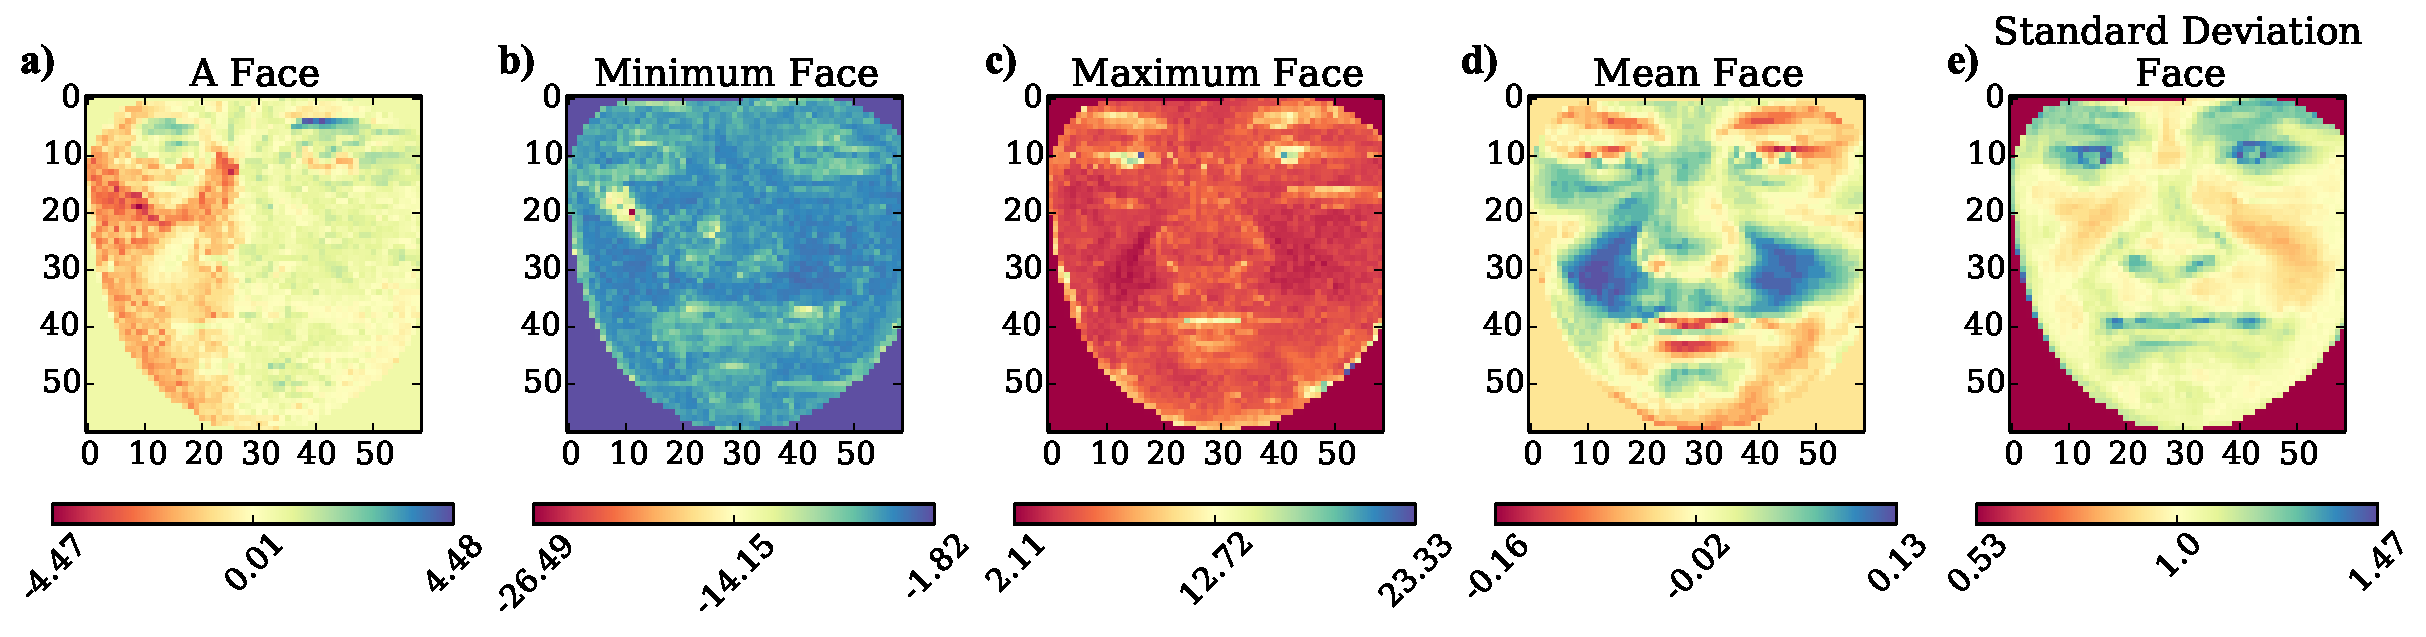
\includegraphics[width =\hsize]{figures/faces_per_subject_contrast_face.pdf}
      \caption{The DISFA dataset with {\bf per subject mean face normalisation and then contrast normalisation} applied.
      Plots {\bf a)}, {\bf b)}, {\bf c)}, {\bf d)} and {\bf e)}
      correspond to a sample face, the minimum, the maximum,
      the mean and the standard deviation values of each pixel across
      the whole dataset. The images were downscaled by a factor of 0.8 before being processed.}
      \label{fig:faces_per_subject_contrast_face} \end{figure}

    %
    %
    %
    %
    %
    \subsection{Masking} \label{sec:mask}
      From figure \ref{fig:faces_none} it is evident some pixels have a maximum and minimum value
      of zero and no deviation. This means there is no information in these areas and hence
      the classifier algorithm would ideally not even know about them. If the network was a set of fully connected layers
      these pixels could just be removed from the system, however convolutional layers require
      rectangular inputs and so a solution is to apply a mask at the level of the cost function.

      This applies only to the autoencoder which has a cost function (equation \ref{eq:autoencoder_cost}):
      \begin{equation}
          J(\tilde{\mathbf{x}},\tilde{\mathbf{y}})
          = \frac{1}{N}\left |\mathbf{y}(\tilde{\mathbf{x}})-\tilde{\mathbf{x}}\right | ^2
      \end{equation}
      Applying masking it becomes:
      \begin{equation}
          J(\tilde{\mathbf{x}},\tilde{\mathbf{y}})
          = \frac{1}{N}\left |\mathbf{y}(\tilde{\mathbf{x}}) \odot \mathbf{M}-\tilde{\mathbf{x}}\right | ^2
      \end{equation}

      Where M is a two dimensional matrix with elements unity where the dataset is non-zero
      and zero when the dataset is zero for that pixel. Here $\odot$ denotes an element-wise
      product between two matrices.

\chapter{Model} \label{sec:model}
  % This chapter describes the path taken in constructing the autoencoding classifier (AEC) network, detailing
  % the experiments which were performed to create the final configuration.
  % The most important metric used to judge a network in the chapter is this Average ROC score of the classifier
  % when applied to the un-seen test set, the secondary metric is the error
  % in the reconstructed image outputted from the autoencoder. The overall aim is to
  % find a configuration where the presence of the autoencoder improves
  % the performance of the classifier and secondarily where improving the secondary metric (the autoencoder) improves
  % the primary metric (the classifier).

  This chapter details the models proposed in order to achieve the aims of the project.
  First a set of common parameters for all models, then a set of possible
  classification structures are defined. Next a set of networks inspired
  by the literature and to span varying complexity.
  Then process of adding a set of regularisation techniques is shown and finally the
  various branch balancing functions are described.

  \section{Common Parameters}
    In order to develop the network for modelling the DISFA dataset a set of common
    parameters for experimentation are useful to define, these are shown in table \ref{tab:common}
    and are assumed unless stated otherwise in the whole chapter.

    \begin{table}[!h]
      \centering { \footnotesize
      \begin{tabular}{ll}
        \hline
        \textbf{Parameter}                       & \textbf{Value}                \\ \hline
        Optimizer                                & Adam                          \\
        Learning Rate                            & $10^{-3}$                     \\
        L2 Regularisation Coefficient            & 0                             \\
        Hidden layer activation functions        & Leaky ReLu, $\alpha=0.01$     \\
        Image downscaling                        & 0.4 ($47\times47$)        \\
        AU's present                             & 1,2,4,5,6,9,12,15,17,20,25,26 \\
        Iterations:                              & 1000                          \\
        Early model save percent                 & 50\%                          \\
        Weight tensor initial standard deviation & $10^{-3}$                     \\
        Bias tensor initial value                & $10^{-2}$                     \\
        Train batch size                         & 100                           \\
        Validation batch size                    & 500                           \\
        Autoencoder cost function                & Mean Squared Error            \\
        Classifier cost function                 & Cross Entropy                 \\
        \hline
      \end{tabular}
      \caption{Common parameters for most experiments in the section. These parameters should be
      assumed in proceeding sections unless otherwise stated.} \label{tab:common} }
    \end{table}

    The Adam optimizer is a popular choice for deep learning models and has an adaptive learning rate
    so the learning rate is initially set to $10^{-3}$ which is standard. The Leaky ReLu
    has shown small improvements in classification rates so is used as opposed
    to the standard ReLU. Images are downscaled by 0.4 to the resolution $47\times47$
    as in done in some of the networks shown in \ref{tab:compnet}
    The early model save percent states when the whole model should be saved early,
    this means for each experiment run there are two models to be evaluated. This
    is useful for the evaluation of both autoencoder and classifier training in one go.

    The mean squared error is chosen to train the autoencoder as there are no alternatives
    and the cross entropy for the classifer it heavily penalises incorrect classifications,
    unlike the mean squared error.

  \section{Joint classification}

    Typical deep neural networks are used to classify
    one image into only one category. The case with FAU detection is different, we
    would like to be able to classify the categories jointly,  putting one frame into more than
    one AU category. Ideally the network would output a confidence score between 0 and 1
    to signify if an AU is present and we would calculate some optimum threshold value
    (ideally this would be 0.5).

    The following list details three possible solutions to the joint classification problem:

    \begin{itemize} \label{sec:binsoft}
      \item {\bf Softmax Layer} - This is a traditional, fully connected layer with
      a softmax activation function (see equation \ref{eq:softmax}).
      The issue with this is that it provides a probability distribution over AUs
      but the required quantity is a probability distribution for each AU.
      \item {\bf Sigmoid Layer} - This again is like the previous solution but instead each neuron gives a confidence
      score between 0 and 1 for each AU with a sigmoid function (see equation \ref{eq:sigmoid}).
      The issue with this however is that sigmoid
      functions have vanishing gradients at large input values
      hence training may become difficult.
      \item {\bf Binary Softmax Layers} - Here there is a two neuron softmax layer
      for each AU, this doubles the amount of weights
      but gives a probability over the presence and
      absence of each AU which is ideal. In the implementation
      the negative neuron of each binary layer is only used for training purposes, and it is
      discarded while evaluating the classification performance.
    \end{itemize}




  \section{Network Structures}

    \begin{figure}[h!]
     \centering
     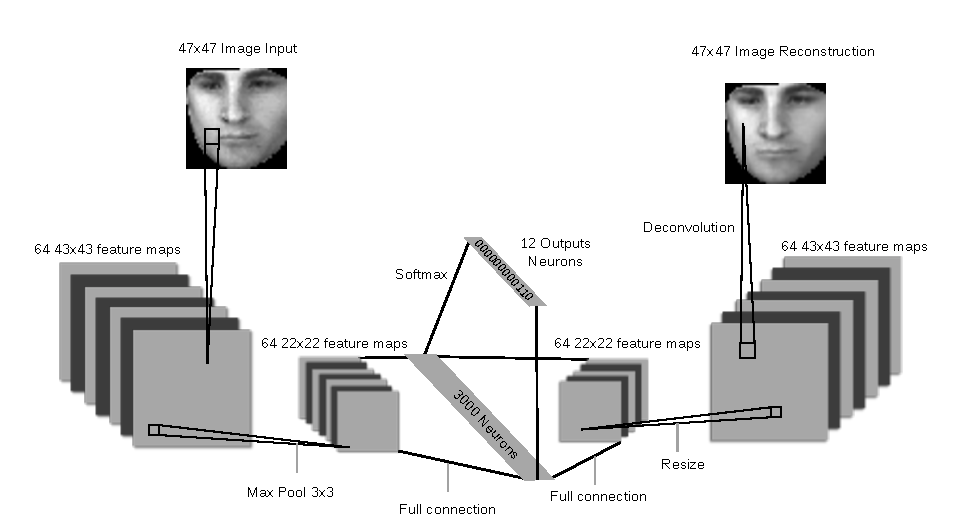
\includegraphics[width=\textwidth]{illustrations/aec_network.pdf}
     \captionof{figure}{A diagram of network 2 used in this section.}
    \end{figure}

    Now that some basic structures have been tested we proceed to convolutional networks,
    inspired by the literature (see table \ref{tab:compnet}) three networks are defined.
    Network \networkII is shown in table \ref{tab:net2}, Network \networkII
    adds another convolutional layer of size $5\times 5 \times 64 \times 64$ to this and
    Network \networkIV adds a $4\times 4 \times 64 \times 128$ layer
    on top of Network \networkII. Regarding the decoder section the inverse operations are
    performed, see appendix \label{appendix1} for full details
    for networks \networkII,\networkII and \networkIV.

    This section shows the network structures used, branching in a network is described
with an extra column.
\begin{table}[h!]
  \caption*{\textbf{Network \networkI}}
	\centering
	{\footnotesize
		\begin{tabular}{|lllllllll|}
			\hline
			\multicolumn{1}{|l|}{Element} & Type    & \multicolumn{1}{l|}{Dimensions}           & Type           & \multicolumn{1}{l|}{Dimensions}            \\ \hline
			\multicolumn{1}{|l|}{x}       &         & \multicolumn{1}{l|}{$47\times47\times1$}  &                & \multicolumn{1}{l|}{}                      \\ \hline
			\multicolumn{1}{|l|}{$L_1$}   & flatten + fc      & \multicolumn{1}{l|}{$2209\times12$}       & Binary Softmax & \multicolumn{1}{l|}{$3000\times2\times12$} \\
			\multicolumn{1}{|l|}{$y_1$}   & dropout & \multicolumn{1}{l|}{$12$}                 &                & \multicolumn{1}{l|}{$24$}                  \\ \hline
			\multicolumn{1}{|l|}{$L_2$}   & fc      & \multicolumn{1}{l|}{$12\times2209$}       &                & \multicolumn{1}{l|}{}                      \\
			\multicolumn{1}{|l|}{$y_2$}   &         & \multicolumn{1}{l|}{$3000$}               &                & \multicolumn{1}{l|}{}                      \\ \hline
			\multicolumn{1}{|l|}{$L_3$}   & reshape & \multicolumn{1}{l|}{}                     &                & \multicolumn{1}{l|}{}                      \\
			\multicolumn{1}{|l|}{$y_3$}   &         & \multicolumn{1}{l|}{$47\times47\times 1$} &                & \multicolumn{1}{l|}{}                      \\ \hline
		\end{tabular}

		\caption{This network is the simplest possible which implements the autoencoder classifier structure.
    It first flattens the input image, runs it through the first layer to get 12 neuron activations.
    Then it branches, for the decoder into a layer of size $2209$ which is reshaped into a $47\times47$ reconstruction and for the classifier into 12 pairs of binary softmax layers.
    *Bottleneck layer} \label{tab:netI}

	}
\end{table}

\begin{table}[h!]
  \caption*{\textbf{Network \networkII}}
	\centering
	{\footnotesize
		\begin{tabular}{|lllllllll|}
			\hline
			\multicolumn{1}{|l|}{Element} & Type             & \multicolumn{1}{l|}{Dimensions}                  & Type   & \multicolumn{1}{l|}{Dimensions}             \\ \hline
			\multicolumn{1}{|l|}{x}       &                  & \multicolumn{1}{l|}{$47\times47\times1$}         &         & \multicolumn{1}{l|}{}                      \\ \hline
			\multicolumn{1}{|l|}{$L_1$}   & conv 1           & \multicolumn{1}{l|}{$5\times 5\times1\times 64$} &         & \multicolumn{1}{l|}{}                      \\
			\multicolumn{1}{|l|}{$y_1$}   &                  & \multicolumn{1}{l|}{$43\times43\times64$}        &         & \multicolumn{1}{l|}{}                      \\ \hline
			\multicolumn{1}{|l|}{$L_2$}   & max pool         & \multicolumn{1}{l|}{$2\times 2$}                 &         & \multicolumn{1}{l|}{}                      \\
			\multicolumn{1}{|l|}{$y_2$}   &                  & \multicolumn{1}{l|}{$22\times22\times 64$}       &         & \multicolumn{1}{l|}{}                      \\ \hline
			\multicolumn{1}{|l|}{$L_3$*}  & fc               & \multicolumn{1}{l|}{$30976\times3000$}           & Binary
                                                                                                            Softmax & \multicolumn{1}{l|}{$3000\times2\times12$} \\
			\multicolumn{1}{|l|}{$y_3$}   & dropout          & \multicolumn{1}{l|}{$3000$}                      &         & \multicolumn{1}{l|}{$24$}                  \\ \hline
			\multicolumn{1}{|l|}{$L_4$}   & fc               & \multicolumn{1}{l|}{$3000\times30976$}           &         & \multicolumn{1}{l|}{}                      \\
			\multicolumn{1}{|l|}{$y_4$}   &                  & \multicolumn{1}{l|}{$3000$}                      &         & \multicolumn{1}{l|}{}                      \\ \hline
			\multicolumn{1}{|l|}{$L_5$}   & resize\& reshape & \multicolumn{1}{l|}{$2$}                         &         & \multicolumn{1}{l|}{}                      \\
			\multicolumn{1}{|l|}{$y_5$}   &                  & \multicolumn{1}{l|}{$43\times43\times 64$}       &         & \multicolumn{1}{l|}{}                      \\ \hline
			\multicolumn{1}{|l|}{$L_6$}   & deconv 1         & \multicolumn{1}{l|}{$5\times 5\times1\times 64$} &         & \multicolumn{1}{l|}{}                      \\
			\multicolumn{1}{|l|}{$y_6$}   &                  & \multicolumn{1}{l|}{$47\times47\times1$}         &         & \multicolumn{1}{l|}{}                      \\ \hline
		\end{tabular}

		\caption{ \newline *Bottleneck layer} \label{tab:netII}
	}
\end{table}

\begin{table}[h!]
	\centering
	\caption*{\textbf{Network \networkIII}}
	{\footnotesize
		\begin{tabular}{|lllllllll|}
			\hline
			\multicolumn{1}{|l|}{Element} & Type             & \multicolumn{1}{l|}{Dimensions}                  & Type           & \multicolumn{1}{l|}{Dimensions}            \\ \hline
			\multicolumn{1}{|l|}{x}       &                  & \multicolumn{1}{l|}{$47\times47\times1$}         &                & \multicolumn{1}{l|}{}                      \\ \hline

			\multicolumn{1}{|l|}{$L_1$}   & conv 1           & \multicolumn{1}{l|}{$5\times 5\times1\times 64$} &                & \multicolumn{1}{l|}{}                      \\
			\multicolumn{1}{|l|}{$y_1$}   &                  & \multicolumn{1}{l|}{$43\times43\times64$}        &                & \multicolumn{1}{l|}{}                      \\ \hline

			\multicolumn{1}{|l|}{$L_2$}   & max pool         & \multicolumn{1}{l|}{$2\times 2$}                 &                & \multicolumn{1}{l|}{}                      \\
			\multicolumn{1}{|l|}{$y_2$}   &                  & \multicolumn{1}{l|}{$22\times22\times 64$}       &                & \multicolumn{1}{l|}{}                      \\ \hline

			\multicolumn{1}{|l|}{$L_3$}   & conv 2           & \multicolumn{1}{l|}{$5\times 5\times1\times 64$} &                & \multicolumn{1}{l|}{}                      \\
			\multicolumn{1}{|l|}{$y_3$}   &                  & \multicolumn{1}{l|}{$18\times18\times64$}        &                & \multicolumn{1}{l|}{}                      \\ \hline

			\multicolumn{1}{|l|}{$L_4$}   & fc               & \multicolumn{1}{l|}{$20736\times3000$}           & Binary Softmax & \multicolumn{1}{l|}{$3000\times2\times12$} \\
			\multicolumn{1}{|l|}{$y_4$}   & dropout          & \multicolumn{1}{l|}{$3000$}                      &                & \multicolumn{1}{l|}{$24$}                  \\ \hline

			\multicolumn{1}{|l|}{$L_5$}   & fc               & \multicolumn{1}{l|}{$3000\times20736$}           &                & \multicolumn{1}{l|}{}                      \\
			\multicolumn{1}{|l|}{$y_5$}   &                  & \multicolumn{1}{l|}{$3000$}                      &                & \multicolumn{1}{l|}{}                      \\ \hline

			\multicolumn{1}{|l|}{$L_6$}   & resize\& reshape & \multicolumn{1}{l|}{$2$}                         &                & \multicolumn{1}{l|}{}                      \\
			\multicolumn{1}{|l|}{$y_6$}   &                  & \multicolumn{1}{l|}{$18\times18\times 64$}       &                & \multicolumn{1}{l|}{}                      \\ \hline

			\multicolumn{1}{|l|}{$L_7$}   & deconv 2         & \multicolumn{1}{l|}{$5\times 5\times1\times 64$} &                & \multicolumn{1}{l|}{}                      \\
			\multicolumn{1}{|l|}{$y_7$}   &                  & \multicolumn{1}{l|}{$22\times22\times64$}        &                & \multicolumn{1}{l|}{}                      \\ \hline


			\multicolumn{1}{|l|}{$L_8$}   & deconv 1         & \multicolumn{1}{l|}{$5\times 5\times1\times 64$} &                & \multicolumn{1}{l|}{}                      \\
			\multicolumn{1}{|l|}{$y_8$}   &                  & \multicolumn{1}{l|}{$47\times47\times1$}         &                & \multicolumn{1}{l|}{}                      \\ \hline
		\end{tabular}
		\caption{ \newline *Bottleneck layer} \label{tab:netIII}
	}
\end{table}

\begin{table}[h!]
	\centering
	\caption*{\textbf{Network \networkIV}}
	{\footnotesize
		\begin{tabular}{|lllllllll|}
			\hline
			\multicolumn{1}{|l|}{Element} & Type             & \multicolumn{1}{l|}{Dimensions}                  & Type           & \multicolumn{1}{l|}{Dimensions}            \\ \hline
			\multicolumn{1}{|l|}{x}       &                  & \multicolumn{1}{l|}{$47\times47\times1$}         &                & \multicolumn{1}{l|}{}                      \\ \hline

			\multicolumn{1}{|l|}{$L_1$}   & conv 1           & \multicolumn{1}{l|}{$5\times 5\times1\times 64$} &                & \multicolumn{1}{l|}{}                      \\
			\multicolumn{1}{|l|}{$y_1$}   &                  & \multicolumn{1}{l|}{$43\times43\times64$}        &                & \multicolumn{1}{l|}{}                      \\ \hline

			\multicolumn{1}{|l|}{$L_2$}   & max pool         & \multicolumn{1}{l|}{$2\times 2$}                 &                & \multicolumn{1}{l|}{}                      \\
			\multicolumn{1}{|l|}{$y_2$}   &                  & \multicolumn{1}{l|}{$22\times22\times 64$}       &                & \multicolumn{1}{l|}{}                      \\ \hline

			\multicolumn{1}{|l|}{$L_3$}   & conv 2           & \multicolumn{1}{l|}{$5\times 5\times1\times 64$} &                & \multicolumn{1}{l|}{}                      \\
			\multicolumn{1}{|l|}{$y_3$}   &                  & \multicolumn{1}{l|}{$18\times18\times64$}        &                & \multicolumn{1}{l|}{}                      \\ \hline

			\multicolumn{1}{|l|}{$L_4$}   & conv 3           & \multicolumn{1}{l|}{$5\times 5\times1\times 64$} &                & \multicolumn{1}{l|}{}                      \\
			\multicolumn{1}{|l|}{$y_4$}   &                  & \multicolumn{1}{l|}{$15\times15\times64$}        &                & \multicolumn{1}{l|}{}                      \\ \hline

			\multicolumn{1}{|l|}{$L_5$}   & fc               & \multicolumn{1}{l|}{$14400\times3000$}           & Binary Softmax & \multicolumn{1}{l|}{$3000\times2\times12$} \\
			\multicolumn{1}{|l|}{$y_5$}   & dropout          & \multicolumn{1}{l|}{$3000$}                      &                & \multicolumn{1}{l|}{$24$}                  \\ \hline

			\multicolumn{1}{|l|}{$L_6$}   & fc               & \multicolumn{1}{l|}{$3000\times 14400$}          &                & \multicolumn{1}{l|}{}                      \\
			\multicolumn{1}{|l|}{$y_6$}   &                  & \multicolumn{1}{l|}{$3000$}                      &                & \multicolumn{1}{l|}{}                      \\ \hline

			\multicolumn{1}{|l|}{$L_7$}   & resize\& reshape & \multicolumn{1}{l|}{$2$}                         &                & \multicolumn{1}{l|}{}                      \\
			\multicolumn{1}{|l|}{$y_7$}   &                  & \multicolumn{1}{l|}{$15\times15\times 64$}       &                & \multicolumn{1}{l|}{}                      \\ \hline

			\multicolumn{1}{|l|}{$L_8$}   & deconv 3         & \multicolumn{1}{l|}{$5\times 5\times1\times 64$} &                & \multicolumn{1}{l|}{}                      \\
			\multicolumn{1}{|l|}{$y_8$}   &                  & \multicolumn{1}{l|}{$18\times18\times64$}        &                & \multicolumn{1}{l|}{}                      \\ \hline

			\multicolumn{1}{|l|}{$L_9$}   & deconv 2         & \multicolumn{1}{l|}{$5\times 5\times1\times 64$} &                & \multicolumn{1}{l|}{}                      \\
			\multicolumn{1}{|l|}{$y_9$}   &                  & \multicolumn{1}{l|}{$22\times22\times64$}        &                & \multicolumn{1}{l|}{}                      \\ \hline


			\multicolumn{1}{|l|}{$L_{10}$}   & deconv 1         & \multicolumn{1}{l|}{$5\times 5\times1\times 64$} &                & \multicolumn{1}{l|}{}                      \\
			\multicolumn{1}{|l|}{$y_{10}$}   &                  & \multicolumn{1}{l|}{$47\times47\times1$}         &                & \multicolumn{1}{l|}{}                      \\ \hline
		\end{tabular}
		\caption{ \newline *Bottleneck layer} \label{tab:netIV}
	}
\end{table}


  \section{Sharing Weights}
    ONLY SHARE THE WEIGHTS BUT SHARE THEM ALL, THE BIASES NAH
    In order to reduce the number of parameters in an autoencoder, to avoid over fitting
    and the probability of learning the identity function, it is often helpful to share weights
    between the encoder and decoder sections.
  \section{Local Contrast Normalisation}
    Local Contrast Normalisation applied differently for each network, as follows:
    \begin{itemize}
      \item
    \end{itemize}
  \section{Dropout}
    A dropout layer was included in all networks at the bottle neck layer.
  \section{L2 Regularisation}
    L2 Regularisation incurs a penalty to using weights which have high values. This was implemented by adding L2
    loss terms for all weight variables. The new cost function becomes:

    \begin{equation} \label{eq:l2_cost_model}
        J(\tilde{\mathbf{x}},\tilde{\mathbf{y}}) = -\frac{1-\alpha(t)}{2FN}\tilde{\mathbf{y}}\cdot\log(\mathbf{y}(\tilde{\mathbf{x}}))
        + \frac{\alpha(t)}{N}\left |\mathbf{y}(\tilde{\mathbf{x}}) \odot \mathbf{M}-\tilde{\mathbf{x}}\right | ^2
        + \beta \sum_i^{\text{weights}}||\mathbf{W}_i||^2
    \end{equation}

    Where $\beta$ is some positive balancing factor and $\mathbf{W}$ signifies
    a weight tensor from any type of layer in the network.



  \section{Autoencoder classifier balancing}
    \label{sec:autoalpha}
    A key structure that is to be investigated in this report is a network with two objective functions:
    autoencoder and classifier. This is achieved by having a bottleneck layer where the branching occurs.
    The autoencoder has symmetry along this bottleneck, while the classifier consists of one further layer
    (the binary softmax classifier from the previous section). The cost function for the whole network is as follows:

    \begin{equation}
      J(\tilde{\mathbf{x}},\tilde{\mathbf{y}}) = -\frac{1-\alpha(t)}{2FN_B}\tilde{\mathbf{y}}\cdot\log(\mathbf{y}(\tilde{\mathbf{x}}))
      + \frac{\alpha(t)}{N_BN_P}\left |\mathbf{y}(\tilde{\mathbf{x}}) \odot \mathbf{M}-\tilde{\mathbf{x}}\right | ^2
    \end{equation}

    Where $\mathbf{M}$ is a mask described in section \ref{sec:mask}. Here F is the number of AU's, N is the size of the batch and $\alpha(t)$ is a
    function which balances the two costs. $\alpha(t)$ might be constant $\left ( \alpha_{\text{constant}}(t)=\frac{1}{2} \right )$ or
    some sort of polynomial which stays in the range $[0,1]$. $N_B$ and $N_P$ are the batch size and number of pixels respectively.

    For much of the initial investigations we employ:
    \begin{equation}
      \alpha_{\text{step}}(t,p,T) =
      \begin{cases}
        1           & \text{if}\ t<pT \\
        0           & \text{otherwise}
      \end{cases}
    \end{equation}

    Where $t$ indexes iterations, $T$ is the total number of iterations and p is the
    percentage of iterations that should be in the first region of the piecewise function
    where $\alpha=1$.
    This nicely expresses what is typically meant by pre-training in the literature, it trains
    the autoencoder up until iteration $pT$ (normally $p=\frac{1}{2}$ or $p=\frac{2}{3}$) and then the classifier for the remainder of the time.
    This acts as a good base case to test both sides of the network, later more interesting
    functions will be explored such as the sigmoid step:

    \begin{equation}
      \alpha_{\text{sigmoid}}(t,T,p,\tau) = \frac{1}{1 + \exp(1 + \tau (t/T - p))}
    \end{equation}

    Or a polynomial function:

    \begin{equation}
      \alpha_{\text{poly}}(t,T,n) = 1 - \left ( \frac{t}{T} \right )^n
    \end{equation}

    Or a periodic step function:

    \begin{equation}
      \alpha_{\text{alternate}}(t,T,p) =
      \begin{cases}
        1           & \text{if } t < |T/p| \text{ and } p > 0\\
        0           & \text{if } t < |T/p| \text{ and } p \leq 0\\
        \alpha_{\text{alternate}}(t-|T/p|,T,-p)           & \text{otherwise} \\
      \end{cases}
    \end{equation}

    Examples of such functions are plotted in figure \ref{fig:alpha_functions}.

    \begin{figure}[!h]
      \centering
      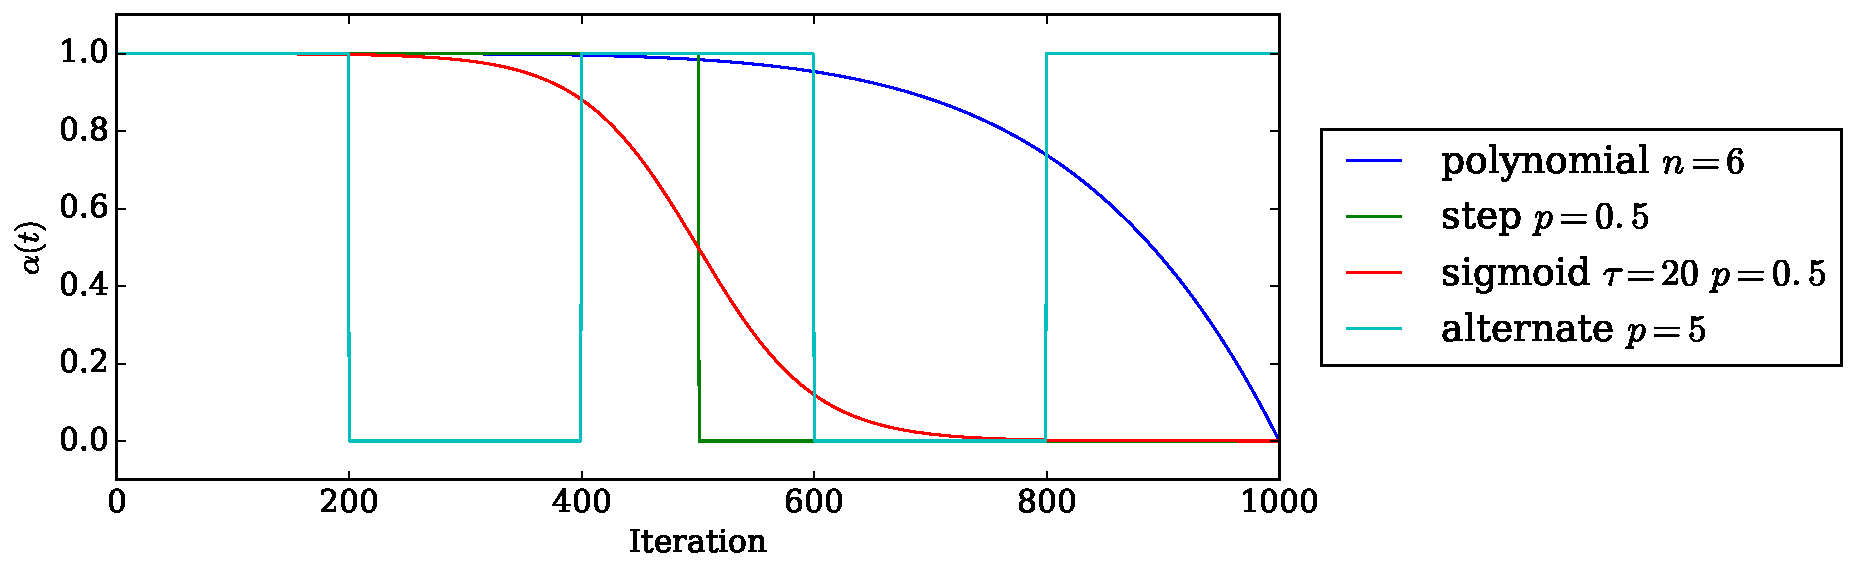
\includegraphics[width =\hsize]{figures/alpha.pdf}
      \caption{Examples of branch balancing functions described in section \ref{sec:autoalpha}.
      For the polynomial case higher values of $n$ decrease the amount of training
      the classifier receives. While in the case of the step p dictates the training
      that each network receives, the sigmoid can be seen as a smoothed out step function
      with the two being equivalent as $ \tau \rightarrow \infty$. Similarly as $n \rightarrow \infty$
      the polynomial function turns into a constant function with $c=1$ except at the final
      iteration.}
      \label{fig:alpha_functions}
    \end{figure}

  \section{Qualitative Results}

\chapter{Evaluation} \label{chap:Evaluation}

  For all of the experiments the data was partitioned in a 50/50 split
  (by subject) as shown in table \ref{tab:splitting}:
  \begin{table}[h!]
    \centering { \footnotesize
    \begin{tabular}{|l|l|}
    \hline
    Set & Subjects   \\
    \hline
     Train          & 2,4,6,8,10,12,16,18,23,25,27,29,31      \\
    \hline
    Validation      & 1,3,5,7,9,11,13,17,21,24,26,28,30,32 minus test set     \\
    \hline
    Test           & 500 chosen randomly taken from validation set      \\
   \hline
    \end{tabular}
    \caption{The split of the DISFA dataset used in the experiments.}
    \label{tab:splitting} }
  \end{table}

  AU intensities 1-5 counted as a positive examples and AU intensity 0 counted as a negative example.
  To calculate autoencoder loss, ROC and F1 values for a trained model, the whole test
  set was run through the network and an average taken.

  To calculate the ROC the \texttt{sklearn} library was used, for the F1 20 thresholds
  between 0 and 1 were used and the best F1 score taken. For the autoencoder
  the losses were standardized by first applying the inverse transforms of the the preprocessing
  methods described in \ref{sec:methods} to the reconstructed images
  and then the mean squared difference was taken.

  \section{A Single Hidden Layer}

    To get a initial baseline reading of what the simplest model can achieve
    network \networkI\ is used. Per subject face normalisation from
    section \ref{sec:meanface} is chosen and the images are scaled with a factor of 1.0
    giving an image size $118 \times 118$.

    \begin{figure}[!h]
    \centering
    \includegraphics[width =\hsize]{../graphs/losses_2016_08_14_004.pdf}
    \caption{The losses of network \networkI\ during training. The $\alpha$ coefficient determines the balance between the
    classifier and the autoencoder losses, $\alpha=1$ signifies only autoencoder training
    while $\alpha=0$ means only classifier training. Over fitting is observed
    on all loss functions. Training the classifier
    overwrites the weights and hence ends up reducing
    the performance of the autoencoder however the
    model is so simple that the validation set remains almost constant.}
    \label{fig:simpleloss}
    \end{figure}

    Overfitting to the train set is evident very
    early in the training from figure \ref{fig:simpleloss},
    this occurs for a number of reasons:
    \begin{itemize}
      \item The model is very simple.
      \item The validation set might not fully represent many AUs and AU combinations possible.
      \item The train and validation sets have no subjects in common with the train set.
            So unless a subject independent model is learnt, a large degree of overfitting will always occur.
    \end{itemize}

    Training the classifier reduces the performance of the autoencoder on the
    training set visibly but interestingly the same is not true for the validation set, meaning
    that the autoencoder failed to learn a general hypotheses. This is
    excepted due to the simplicity of the model.

    \begin{table}[!h]
    \centering
    {\small
    \begin{tabular}{llllll}
    \hline
    \textbf{Class}    & \textbf{ROC} & \textbf{ROC Ranking} & \textbf{Max F1} & \textbf{Max Precision} & \textbf{Max Recall} \\ \hline
    1                 & 0.50  & fail  & 0.09  & 0.06    & 1.0      \\
    2                 & 0.60  & poor  & 0.07  & 0.05    & 1.0      \\
    4                 & 0.62  & poor  & 0.31  & 0.27    & 1.0      \\
    5                 & 0.49  & fail  & 0.02  & 0.02    & 1.0      \\
    6                 & 0.80  & fair  & 0.48  & 0.42    & 1.0      \\
    9                 & 0.46  & fail  & 0.11  & 0.06    & 1.0      \\
    12                & 0.89  & good  & 0.67  & 0.73    & 1.0      \\
    15                & 0.46  & fail  & 0.11  & 0.06    & 1.0      \\
    17                & 0.55  & fail  & 0.18  & 0.25    & 1.0      \\
    20                & 0.51  & fail  & 0.09  & 0.12    & 1.0      \\
    25                & 0.65  & poor  & 0.51  & 0.42    & 1.0      \\
    26                & 0.57  & fail  & 0.32  & 0.23    & 1.0      \\ \hline
    \textbf{Average:} & 0.59  & fail  & 0.25  & 0.22    & 1.0      \\ \hline
    \end{tabular} }
    \caption{The final evaluation for the training session shown in \ref{fig:simple}.
    AU 12 and 6 are the only AUs learnt well. These values were
    calculated on the test set. The maximum F1s, precisions and recalls
    were found by trying 20 threshold values between 0 and 1.}
    \label{tab:biglist}
    \end{table}

    Table \ref{tab:biglist} shows finally the scores for each AU, although as expected
    most AUs fail, this table shows the values that are normally averaged in the following sections
    and so is instructive to display early in the evaluation section.

  \clearpage
  \section{Joint Classification}
    Table \ref{tab:binsoftcomp} compares how each of the solutions from section \ref{sec:joints}
    perform in a network using mean face normalisation (not per subject) and using the network
    \networkII\
    , this network was chosen because it contains all of the
    main components of larger networks typically used for classification tasks,
    such as a convolutional layer, max pool layer and fully connected layer.
    % ID = 4 date = '2016_08_14' group = 'alpha'

    \begin{table}[!h]
        {\footnotesize
        \centering
        \begin{tabular}{lccc}
        \hline
        Final Layer   & Av. ROC &   Av. Best F1 &   Autoencoder Loss (Not normalised) \\
        \hline
        Binary Softmax Layers  &   0.73 &  0.34 &   20.7 \\
        Softmax Layer          &   0.69 &  0.30 &   15.8 \\
        Sigmoid Layer          &   0.50 &  0.19 &  126.2 \\
        \hline
        \end{tabular}
      \caption{Comparison of the three ways the final layer could be implemented
      using \networkII\ (see table \ref{tab:netII}). The
      preprocessing method used was face normalisation (not per subject).
      500 iterations were used. }
      \label{tab:binsoftcomp}
      }
      \end{table}

      The results show that the binary softmax layer outperforms the other
      solutions. The softmax layer is only slightly worse, but in order to
      accommodate for the potential of higher classification rates it is in
      theory also clear that the binary
      softmax is the better choice. This is because, in joint classification
      problems the simple softmax layer struggles to report more than 2 AUs as
      the outputs must add up to one. The low performance of the sigmoid layer
      is interesting and one reason might be that of vanishing gradients due to
      the bottleneck layer (which feeds into the final layer) containing high activation values.

      As the softmax layer is better in the results and has a better potential for good results
      it is chosen as the classifier for the following experiments.

      \section{Preprocessing methods} \label{sec:psearch}

          A comparison of the preprocessing methods from section
          \ref{sec:methods} and on the four main activation functions
          that are typically used on the last layer of an autoencoder
          (linear, ReLU, sigmoid and tanh) was performed,
          table \ref{tab:psearch} shows the results.

          These parameters cover a lot of possible
          configurations and should have markedly different results, the idea
          is that the encoding at the bottleneck layer should be different for
          each set of parameters and that
          one of these might offer a good starting set of weights for the
          classifier to train from. What is typically meant by this is, is that
          the autoencoder has learnt to pick out some useful features, which the classifier
          can then build on.

          \begin{table}[!h] {\footnotesize
            \centering
          \begin{tabular}{lllrrrrrr}
                && &   \multicolumn{3}{|c|}{Autoencoder Training} &  \multicolumn{3}{c|}{Classifier Training}    \\
            \hline
             i&Preprocessing    & Activation Function&  ROC&F1&AE Loss & ROC & F1 & AE Loss \\
             \hline
             1&Per Subject Contrast Face & linear &    0.49 &   0.19 &     0.12 &    0.82 &   0.46 &     0.18 \\
             2&Per Subject Contrast Face & tanh   &    0.49 &   0.19 &     0.12 &    0.82 &   0.46 &     0.13 \\
             3&Per Subject Contrast Face & relu   &    0.63 &   0.19 &     0.12 &    0.81 &   0.44 &     0.14 \\
             4& Per Subject Contrast Face & sigmoid &    0.52 &   0.2  &     0.13 &    0.08 &   0.19 &     0.13 \\
             \hline
             5&Contrast          & linear &    0.40 &   0.19 &     0.19 &    0.74 &   0.34 &     1.46 \\
             6&Contrast          & tanh   &    0.61 &   0.19 &     0.20 &    0.72 &   0.35 &     0.35 \\
             7&Contrast          & relu   &    0.59 &   0.19 &     0.25 &    0.75 &   0.36 &     0.65 \\
             8& Contrast         & sigmoid &    0.54 &   0.19 &     0.22 &    0.50    &   0.19 &     0.28 \\
             \hline
             9&Face              & linear &    0.46 &   0.19 &     0.06 &    0.73 &   0.35 &     0.26 \\
             10&Face              & tanh   &    0.52 &   0.19 &     0.08 &    0.74 &   0.35 &     0.13 \\
             11&Face              & relu   &    0.45 &   0.19 &     0.09 &    0.73 &   0.36 &     0.35 \\
             12& Face             & sigmoid &    0.47 &   0.2  &     0.1  &    0.72 &   0.35 &     0.13 \\
             \hline
             \hdashline
             13&Per Subject Face  & linear &    $0.64$ &   $0.19$ &     $0.03$ &    $0.83$ &   $0.48$ &     $0.12$ \\
             &{\it error:}  &&$\pm$0.02 &$\pm$0.01 &$\pm$0.02  &$\pm$0.02 &$\pm$0.01 &$\pm$0.02 \\
             \hdashline
             14&Per Subject Face  & tanh   &    0.56 &   0.19 &     0.03 &    0.81 &   0.47 &     0.05 \\
             15&Per Subject Face  & relu   &    0.56 &   0.19 &     0.04 &    0.81 &   0.48 &     0.11 \\
             16& Per Subject Face      & sigmoid &    0.62 &   0.23 &     0.04 &    0.81 &   0.46 &     0.05 \\
             \hline
             17&Range [-1,1]      & linear &    0.50 &   0.19 &     0.07 &    0.73 &   0.35 &     3.90 \\
             18&Range [-1,1]      & tanh   &    0.54 &   0.19 &     0.07 &    0.75 &   0.35 &     0.30 \\
             19&Range [-1,1]      & relu   &    0.48 &   0.19 &     0.15 &    0.73 &   0.35 &     4.73 \\
             20& Range [-1,1]      & sigmoid &    0.49 &   0.2  &     0.12 &    0.73 &   0.31 &     0.36 \\
             \hline
             21&None              & linear &    0.51 &   0.19 &     0.08 &    0.74 &   0.34 &     4.02 \\
             22&None              & tanh   &    0.59 &   0.19 &     0.07 &    0.71 &   0.33 &     0.93 \\
             23&None              & relu   &    0.53 &   0.19 &     0.20 &    0.53 &   0.23 &     0.41 \\
             24& None       & sigmoid &    0.47 &   0.19 &     0.09 &    0.65 &   0.29 &     0.46 \\
             \hline
             25&Contrast Face     & linear &    0.56 &   0.19 &     0.24 &    0.74 &   0.35 &     0.40 \\
             26&Contrast Face     & tanh   &    0.54 &   0.19 &     0.24 &    0.75 &   0.38 &     0.26 \\
             27&Contrast Face     & relu   &    0.54 &   0.19 &     0.25 &    0.74 &   0.35 &     0.35 \\
             28& Contrast Face    & sigmoid &    0.44 &   0.19 &     0.25 &    0.71 &   0.34 &     0.26 \\
             \hline
            \end{tabular}
              \caption{Comparison of four activation functions for the autoencoder for each type of preprocessing method.
              Error values are required because TensorFlow does implement fully deterministic
              processing with GPU cards (see section \ref{sec:GPU} the values in the errors were
              calculated by rerunning experiment 13 5 times. The autoencoder losses were calculated
              by first applying the inverse transform of the preprocessing method and then taking the mean squared
              difference between the reconstructed image and original image. {\bf Experimental Configuration:}
              The alpha function is $\alpha(t)=\alpha_{\text{step}}(t,0.5,1000)$.
              meaning the autoencoder training runs for 500 iterations and then the classifier for 500.
              The network used is \networkII.}
          \label{tab:psearch} }
          \end{table}

          No significant difference is seen between the activation functions apart from with the sigmoid
          which makes training the classifier fail completely.

          The highest ROC and F1 score is found in experiment 13 in table \ref{tab:psearch}. Experiment 12
          has effectively the same score and a lower final autoencoder loss, but it uses the tanh activation
          function and hence cannot fully reconstruct the input image which has values well outside the
          range $[-1,1]$ hence the linear activation function is chosen to ensure the potential for full reconstruction is there.
          Also since this preprocessing method tries to correlate high activation values with AU occurrences, these high values should be
          an important focus of the reconstruction, the tanh functions might focus more on the smaller values which
          do not encode as much AU information.

        %
        %
        %
        %
        %
        \newpage
        \section{Shared Weights}

          Table \ref{tab:sharedweights} shows
          for three networks the effect of having and not having shared weights.

          \begin{table}[!h] \centering
          {\footnotesize
          \begin{tabular}{rrllrrrrrrrr}
            &&&&   \multicolumn{3}{|c|}{Autoencoder Training} &  \multicolumn{3}{c|}{Classifier Training}    \\
          \hline
            i & Network               &   Shared Weights &    ROC&F1&AE Loss & ROC & F1 & AE Loss \\
          \hline
           1 & \networkII    & False     &    0.38 &   0.19 &     0.03 &    0.79 &   0.45 &     0.05 \\
           2 & \networkII    & True      &    0.48 &   0.19 &     0.02 &    0.81 &   0.48 &     0.12 \\
          \hline
          4 & \networkIII    & False     &    0.55 &   0.19 &     0.03 &    0.78 &   0.41 &     0.06 \\
          5 & \networkIII    & True      &    0.56 &   0.19 &     0.02 &    0.8  &   0.46 &     0.18 \\
          \hline
          8 & \networkIV     & False     &    0.54 &   0.19 &     0.03 &    0.77 &   0.38 &     0.05 \\
          9 & \networkIV     & True      &    0.42 &   0.19 &     0.03 &    0.78 &   0.42 &     1.37 \\
           \hline
         \end{tabular}}
             \caption{A simple experiment showing that using shared weights is beneficial
             to both autoencoder loss and classification performance. {\bf Experimental Configuration:}
             The alpha function is $\alpha(t)=\alpha_{\text{step}}(t,0.5,1000)$.
             meaning the autoencoder training runs for 500 iterations and then the classifier for 500.
             The network is described in table \ref{tab:netII}.} \label{tab:sharedweights}
         \end{table}

          It can be seen that using shared weights consistently improves the classification
          performance by a small amount and in some cases the autoencoder performance.
          This could for a number of reasons:
          \begin{itemize}
            \item The more constrained (few parameters) model acts as a good base for classification training
            \item The model learnt without shared weights resembles the identity function and hence is not useful for classification
          \end{itemize}

          In the case of shared weights, the classifier has influence on the weights
          inside of the decoder section, hence as expected in these cases the autoencoder
          is damaged.

          These finding suggest it is useful to include shared weights in a model.
        %
        %
        %
        %
        %
        \newpage
        \section{Local Contrast Normalisation}

          The local contrast normalisation (LRN) scheme
          as described in section \ref{sec:lrn}
          was applied to the three test networks.

          Since some networks can have more than one LRN layer, the effect of
          using some LRN deeper in the network is also tested.

          \begin{table}[!h] \centering
            \footnotesize{
            \begin{tabular}{rrllrrrrrrrr}
              &&&   \multicolumn{3}{|c|}{Autoencoder Training} &  \multicolumn{3}{c|}{Classifier Training}    \\
            \hline
              i & Network             & LRN Layers   &    ROC&F1&AE Loss & ROC & F1 & AE Loss \\
            \hline
             1 & \networkII & 0  &    0.48 &   0.19 &     0.02 &    0.81 &   0.48 &     0.12 \\
             2 & \networkII & 1  &    0.49 &   0.19 &     0.02 &    0.81 &   0.47 &     0.13 \\
            \hline
             3 & \networkIII & 0  &    0.56 &   0.19 &     0.02 &    0.8  &   0.46 &     0.18 \\
             4 & \networkIII & 1  &    0.57 &   0.19 &     0.02 &    0.8  &   0.46 &     0.19 \\
             5 & \networkIII & 2  &    0.52 &   0.19 &     0.02 &    0.8  &   0.45 &     0.22 \\
            \hline
             6 & \networkIV & 0  &    0.42 &   0.19 &     0.03 &    0.78 &   0.42 &     1.37 \\
             7 & \networkIV & 1  &    0.52 &   0.19 &     0.03 &    0.79 &   0.44 &     1.02 \\
             8 & \networkIV & 2  &    0.52 &   0.19 &     0.03 &    0.8  &   0.44 &     0.88 \\
            \hline
            \end{tabular}}

            \caption{Results for applying local contrast normalisation layers
            for the three test networks. LRN Layers 0 means no LRN, 1 means a LRN layer is added after the max pool
            and 2 means a LRN layer is added at the final convolutional layer in the encoder. There is no
            inverse for LRN and hence the decoder section remains unchanged. {\bf Experimental Configuration:} see caption
            for table \ref{tab:sharedweights}
            }
            \label{tab:lrn}
          \end{table}

          Table \ref{tab:lrn} shows that LRN provides some improvement in performance for network 4 and seems
          not to effect the other networks by much. It is interesting that the larger network
          is less likely to reduce autoencoder loss with the LRN layers.

          For these reasons, as LRN seems to improve the bigger networks performance it
          would be good to include in the final model.

          \newpage
        %
        %
        %
        %
        %
        %
        \newpage
        \section{Dropout}
          Varying degrees of dropout (see section \ref{sec:dropout}) were applied to each convolutional
          network at the bottleneck layer.
          Table \ref{tab:dropout} shows the results.
          \begin{table}[h]
          \centering
          { \footnotesize
          \begin{tabular}{rllrrrrrrrr}
                               &         &                                                                                   &                                                                                  & \multicolumn{1}{r|}{} & \multicolumn{3}{c|}{Autoencoder Training}                          & \multicolumn{3}{c|}{Classifier Training}                           \\ \hline
          i                    & network & \multirow{2}{*}{\begin{tabular}[c]{@{}l@{}}Autoencoder\\ Iterations\end{tabular}} & \multirow{2}{*}{\begin{tabular}[c]{@{}r@{}}Classifier\\ Iterations\end{tabular}} & Dropout                    & ROC                  & F1                   & AE Loss              & ROC                  & F1                   & AE Loss              \\
          \multicolumn{1}{l}{} &         &                                                                                   &                                                                                  & \multicolumn{1}{l}{}  & \multicolumn{1}{l}{} & \multicolumn{1}{l}{} & \multicolumn{1}{l}{} & \multicolumn{1}{l}{} & \multicolumn{1}{l}{} & \multicolumn{1}{l}{} \\ \hline
          1                    & \networkII       & 1000              & 500     & 1        & 0.49     & 0.19      & 0.02      & 0.8                  & 0.47                 & 0.12                 \\
          2                    & \networkII       & 1000             & 500       & 0.9      & 0.49     & 0.19      & 0.03      & 0.8                  & 0.47                 & 0.11                 \\
          3                    & \networkII       & 1000             & 500       & 0.8      & 0.52     & 0.19      & 0.03      & 0.82                 & 0.48                 & 0.08                 \\
          4                    & \networkII       & 1000             & 1000       & 0.8      & 0.52     & 0.19      & 0.03      & 0.8                  & 0.46                 & 0.11                 \\
          \hline
          5                    & \networkIII       & 1000             & 500       & 1        & 0.51     & 0.19      & 0.02      & 0.81                 & 0.46                 & 0.21                 \\
          6                    & \networkIII       & 1000             & 500       & 0.9      & 0.51     & 0.19      & 0.02      & 0.81                 & 0.46                 & 0.25                 \\
          7                    & \networkIII       & 1000             & 500       & 0.8      & 0.49     & 0.19      & 0.03      & 0.82                 & 0.46                 & 0.13                 \\
          6                    & \networkIII       & 1000             & 1000       & 0.8      & 0.57     & 0.19      & 0.02      & 0.81                 & 0.44                 & 0.33                 \\
          \hline
          9                    & \networkIV       & 1000             & 500       & 1        & 0.6      & 0.19      & 0.03      & 0.78                 & 0.42                 & 1.03                 \\
          10                   & \networkIV       & 1000             & 500       & 0.9      & 0.63     & 0.19      & 0.03      & 0.71                 & 0.35                 & 0.15                 \\
          11                   & \networkIV       & 1000             & 500       & 0.8      & 0.5      & 0.19      & 0.03      & 0.73                 & 0.36                 & 0.08\\
          12                   & \networkIV       & 1000             & 1000       & 0.8      & 0.52      & 0.19      & 0.03      & 0.77   & 0.38     & 1.01\\
          \hline
          \end{tabular}
          }
          \caption{12 experiments which investigate the affect of applying dropout to the
          three test networks, autoencoder iterations is how many iterations
          the autoencoder is trained for and classifier iterations is for how many
          iterations the
          classifier is then trained. The dropout value represents the
          fraction of neurons which are kept active in the bottleneck layer of each network.
          {\bf Experimental Configuration:} see caption for table \ref{tab:sharedweights}.}
          \label{tab:dropout}
          \end{table}

          All networks are trained with the same number of iterations but they are of very different sizes,
          hence this analysis should not be seen fully as a comparison between networks,
          but a comparison between different amounts of dropout for each network.

          More dropout had little effect on the ROC for networks 2 and 3, however it does
          improve the final loss of the autoencoder. For network 4 the dropout actually decreases
          ROC performance, but again allows the autoencoder to remain more functional.
          The fact that the autoencoder is protected
          agrees with the general idea that any form of regularisation will inhibit large changes
          in weights and encourage less complex models, i.e. it should be easier for the classifier to try and learn
          a representation based on what the autoencoder was doing, instead of replacing it with a completely unrelated
          representation. Another explanation is that the autoencoder
          actually learns a representation which is more helpful for the classifier. This second hypothesis is
          however difficult to prove from the results as the autoencoder losses seem to not be affected by the dropout rate.

          In fact the autoencoder loss seems to have saturated around 0.02-0.03 which
          is an interesting result.

          Experiments 4,6 and 12 show that networks 2 and 3 are almost fully
          trained with 500 iterations as adding more iterations does little
          (even reducing the performance somewhat, but not more than is
          statistically relevant because these values still in have an error).

          To conclude, dropout should be included in the final model as it improves
          classification performance in most cases.

        \newpage
        %
        %
        %
        %
        %
        %
        \section{L2 Regularisation}

          Table \ref{tab:l2_1} shows some experiments which vary $\beta$ (described in sections \ref{sec:modl2} and \ref{sec:bacl2}), they reveal an
          interesting trend, where the ROC and F1 are reduced by L2 losses but the autoencoding
          ability is protected by the L2 loss term. Furthermore the L2 loss term acts
          to bring the cross entropy losses (CEL) of the validation set and train set closer together as can be seen in the table.

          \begin{table}[!h] {\footnotesize \centering
          \begin{tabular}{lrrrrrrrrrrr}
              &&&   \multicolumn{3}{|c|}{Autoencoder Training} &  \multicolumn{5}{c|}{Classifier Training}  \\
            \hline
             i & $\beta$ &   Iterations &   ROC&F1&AE Loss & ROC & F1 & AE Loss &   Validation CEL &   Train CEL \\
            \hline
             1 &     0     & 1000 &    0.45 &   0.19 &     0.03 &    0.77 &   0.46 &     0.11 &  0.53 &  0.07 \\
             2 &     0.001 & 1000 &    0.56 &   0.19 &     0.03 &    0.74 &   0.41 &     0.05 &  0.46 &  0.11 \\
             3 &     0.01  & 1000 &    0.45 &   0.19 &     0.03 &    0.71 &   0.36 &     0.04 &  0.33 &  0.18 \\
             4 &     0.1   & 1000 &    0.54 &   0.19 &     0.04 &    0.66 &   0.28 &     0.04 &  0.3  &  0.26 \\
             5 &     0.5   & 1000 &    0.5  &   0.19 &     0.04 &    0.46 &   0.19 &     0.04 &  0.32 &  0.33 \\
            \hline
          \end{tabular}
            \caption{The experimental set up is the same as in section \ref{sec:psearch} where the preprocessing methods
            were tested, except a slightly earlier version
            of the code was used and hence different ROC and F1 numbers.
            The results should still hold relative to each other.
            CEL (Cross Entropy Loss) is included here to get an idea of how different
            the losses between the validation batches are (of course the
            train batch is just 100 frames, however inspecting figure \ref{fig:l2_1} shows that
            these 100 frames are typically representative enough to draw conclusions from), these
            CEL values are therefore equivalent to the final data points in figure \ref{fig:l2_1}. } \label{tab:l2_1}
          }
          \end{table}

        Table \ref{tab:l2_2} then takes experiments 1 and 4 from table \ref{tab:l2_1} and doubles
        the amount of iterations for both the autoencoder and classifier trainings. It shows
        that the extra iterations can undo the performance loss that the L2 regularisation
        introduces while also still protecting the functionality of the autoencoder.
        This shows in general that L2 is a helpful thing to include in the setting of the autoencoder
        and classifier.

        \begin{table}[!h]
          {\footnotesize \centering
          \begin{tabular}{lrrrrrrrrrrr}
            &&&   \multicolumn{3}{|c|}{Autoencoder Training} &  \multicolumn{3}{c|}{Classifier Training}    \\
          \hline
           i &   $\beta$ &   Iterations &   ROC&F1&AE Loss & ROC & F1 & AE Loss \\
          \hline
           1 &       0.1 & 2000 &    0.56 &   0.19 &     0.03 &    0.74 &   0.35 &     0.04\\
           2 &       0   & 2000 &    0.46 &   0.19 &     0.03 &    0.77 &   0.45 &     0.15\\
          \hline
        \end{tabular}
        \caption{Identical to \ref{tab:l2_1} except with more iterations to investigate what happens with further training.
        The autoencoder and classifier are both trained for 1000 iterations.}
        \label{tab:l2_2} }
        \end{table}

        \begin{figure}[!h]
          \centering
            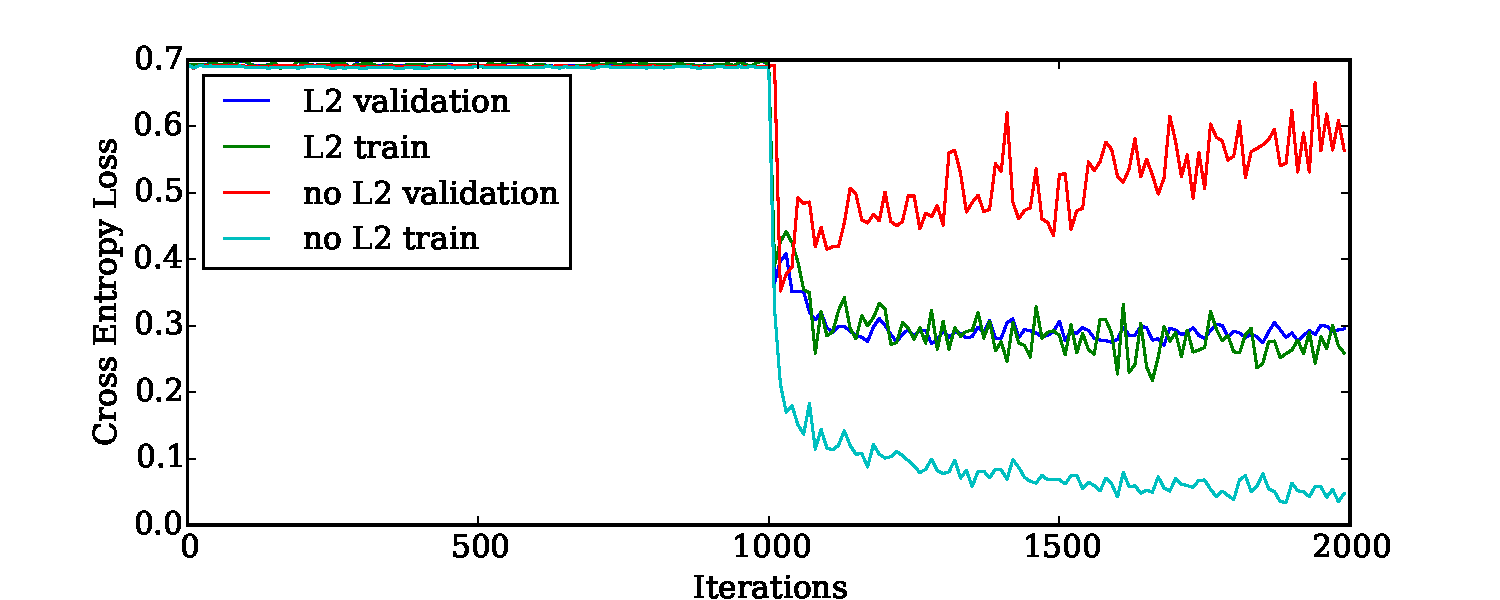
\includegraphics[width =0.8\hsize]{figures/l2.pdf}
              \caption{Plot of the classifier cross entropy losses of the two experiments in table \ref{tab:l2_2} during training.}
          \label{fig:l2_1}
        \end{figure}

        \begin{figure}[!h]
          \centering
            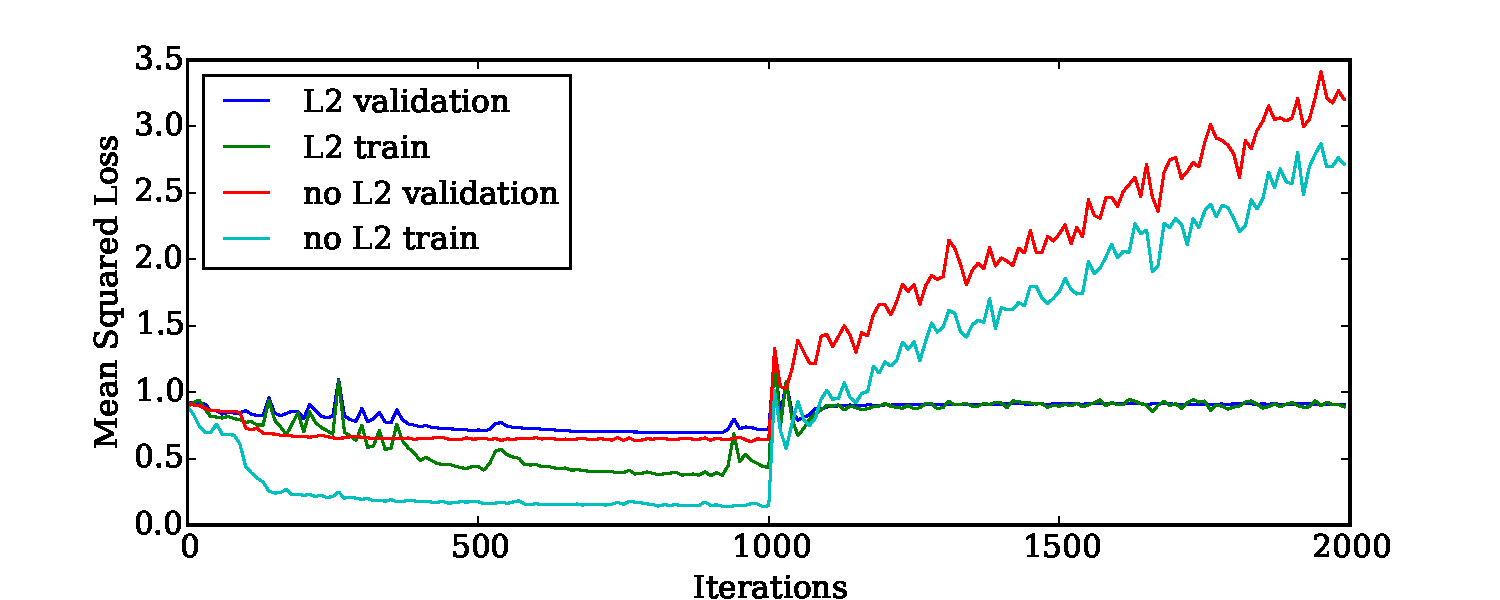
\includegraphics[width =0.8\hsize]{figures/l2_auto.pdf}
              \caption{Plot of the autoencoder mean squared loss of the two experiments in table \ref{tab:l2_2} during training.}
          \label{fig:l2_2}
        \end{figure}

        With these results then, the conclusion is that including a small degree of L2
        Regularisation should be useful for exploring the aims of this project.
        However as there is no significant improvement in classification performance
        and training takes longer it is not included in the final model.


        %
        %
        %
        %
        %
        %
      \section{Autoencoder classifier balancing functions}
        This section investigates the autoencoder balance functions described in section \ref{sec:autoalpha}.
        In addition to these, the classifier only ($\alpha(t) = 0$) are included as a baseline from which to compare
        what the autoencoder actually changes. The experimental question being asked here
        is whether the inclusion of the autoencoder can improve classification performance within the 1500 iterations
        that the network is trained for.



        \begin{table}[]
          \footnotesize{
          \centering
          \begin{tabular}{rrrrrrrrrrr}
                               &                      &                                                                              &                                                                              & \multicolumn{1}{r|}{}                                                       & \multicolumn{3}{c|}{Early Model}                                   & \multicolumn{3}{c|}{Final Model}                                   \\ \hline
          i                    & Network              & \multirow{2}{*}{\begin{tabular}[c]{@{}r@{}}Balance \\ Function\end{tabular}} & \multirow{2}{*}{\begin{tabular}[c]{@{}r@{}}Total \\ Iterations\end{tabular}} & \multirow{2}{*}{\begin{tabular}[c]{@{}r@{}}Early \\ Iteration\end{tabular}} & ROC                  & F1                   & AE Loss              & ROC                  & F1                   & AE Loss              \\
          \multicolumn{1}{l}{} & \multicolumn{1}{l}{} &                                                                              &                                                                              &                                                                             & \multicolumn{1}{l}{} & \multicolumn{1}{l}{} & \multicolumn{1}{l}{} & \multicolumn{1}{l}{} & \multicolumn{1}{l}{} & \multicolumn{1}{l}{} \\ \hline
          2.5                  & \networkII                    & constant 0.0         & 1500           & 1000    & 0.8   & 0.47 & 0.56  & 0.79 & 0.46 & 0.64  \\
          2.3                  & \networkII                    & constant 0.5         & 1500           & 750     & 0.81  & 0.48 & 0.03  & 0.8  & 0.46 & 0.03  \\
          2.1                  & \networkII                    & step                 & 1500           & 1000    & 0.59  & 0.19 & 0.03  & 0.82 & 0.47 & 0.08  \\
          2.4                  & \networkII                    & sigmoid              & 1500           & 1000    & 0.8   & 0.46 & 0.03  & 0.79 & 0.46 & 0.03  \\
          2.6                  & \networkII                    & polynomial           & 1500           & 750     & 0.79  & 0.46 & 0.03  & 0.77 & 0.44 & 0.03  \\
          2.2                  & \networkII                    & alternate            & 1500           & 1000    & 0.81  & 0.46 & 0.1   & 0.82 & 0.47 & 0.12  \\
          \hline
          3.5                  & \networkIII                   & constant 0.0         & 1500           & 1000    & 0.81  & 0.43 & 2.38  & 0.79 & 0.42 & 2.61  \\
          3.2                  & \networkIII                   & constant 0.5         & 1500           & 750     & 0.81  & 0.46 & 0.03  & 0.81 & 0.46 & 0.03  \\
          3.1                  & \networkIII                   & step                 & 1500           & 1000    & 0.38  & 0.19 & 0.03  & 0.81 & 0.45 & 0.18  \\
          3.3                  & \networkIII                   & sigmoid              & 1500           & 1000    & 0.8   & 0.46 & 0.03  & 0.8  & 0.44 & 0.04  \\
          3.4                  & \networkIII                   & polynomial           & 1500           & 750     & 0.78  & 0.45 & 0.02  & 0.79 & 0.44 & 0.03  \\
          3.6                  & \networkIII                   & alternate            & 1500           & 1000    & 0.69  & 0.32 & 0.1   & 0.77 & 0.37 & 0.23  \\
          \hline
          4.1                  & \networkIV                    & constant 0.0         & 1500           & 1000    & 0.78  & 0.38 & 16.31 & 0.78 & 0.39 & 14.5  \\
          4.3                  & \networkIV                    & constant 0.5         & 1500           & 750     & 0.73  & 0.33 & 0.03  & 0.75 & 0.36 & 0.03  \\
          4.2                  & \networkIV                    & step                 & 1500           & 1000    & 0.42  & 0.19 & 0.03  & 0.77 & 0.4  & 0.7   \\
          4.4                  & \networkIV                    & sigmoid              & 1500           & 1000    & 0.74  & 0.36 & 0.03  & 0.74 & 0.36 & 0.03  \\
          4.5                  & \networkIV                    & polynomial           & 1500           & 750     & 0.52  & 0.21 & 0.09  & 0.67 & 0.3  & 0.04  \\
          4.6                  & \networkIV                    & alternate            & 1500           & 1000    & 0.6   & 0.26 & 0.06  & 0.61 & 0.27 & 0.07  \\
          \hline
          \end{tabular}
          }
          \caption{Sorted by ROC performance and secondarily by autoencoder loss.
          A comparison of the the autoencoder balance functions with 0.8 dropout and local contrast normalisation layers (one for network 2 and two for networks 3 \& 4).
          Constant 0.5 means each cost function is trained equally, while constant 0.0 means training only of the classifier.
          Early model is just the evaluation at the early iteration and the final model is the evaluation of the network at the total number of iterations.
          The step function has its step at iteration 1000.
          The sigmoid function is $\alpha_{\text{sigmoid},1500,2/3,20}$
          The polynomial function is $\alpha_{\text{poly},1500,6}$.
          The alternate function is $\alpha_{\text{alternate}}(t,15000,2/3)$
          {\bf Experimental Configuration:} see caption for table \ref{tab:sharedweights}.} \label{tab:auto_final_1}
        \end{table}

          The first thing to note from the results in table \ref{tab:auto_final_1} is that
          the constant 0.0 experiments leave the autoencoder in a particularly dysfunctional state (with losses between 0.64 to 14.5),
          getting worse with the size of the network. Then there is the observation that
          the ROC scores are fairly close, with the F1 scores being almost the same. These two
          observations show that the two networks are achieving a very similar performance but
          with very different configurations. One explanation may be that the binary softmax layer weights
          contain a lot of information about classifying the AU's, if so then this suggests an
          instructive experiment for future work would be to only train these softmax weights to see
          what their maximum performance is. If they can achieve similar results then it may be possible
          the underlying convolution and max pooling layers are not fully helping to model the data.

          There is no obvious evidence that the smoother alpha functions contribute different
          dynamics. In these experiments, one possible issue is that
          the total amount of classifier and autoencoder training is not constant
          \footnote{In other words the area under the $\alpha(t)$ and $1-\alpha(t)$ curves are not constant between runs.}
          between balance functions
          and this is something that might be critical for a really precise exposition. However the question of whether
          including the autoencoder is beneficial is still answerable.

          % [('polynomial', 6), ('alternate', 7), ('sigmoid', 10), ('constant 0.0', 10), ('constant 0.5', 13), ('step', 17)]
          Ranking the functions by their position in table \ref{tab:auto_final_1} scoring 6 for top place and 1 for worst place gives in order:
          step(17), constant 0.5 (13), constant 0.0 (10), sigmoid (10) and lastly alternate (7). Initially this indicates that the
          experiments including the autoencoder perform better but looking at the early models of the constant 0.0 experiments
          they often have very similar performance scores, so the autoencoder improves the performance by stalling the training.

          The losses for network 2 are plotted in appendix \ref{appendix2}, they show for each
          balance function the losses on the autoencoder and classifier.
          They show that the alternate balancing and constant 0.0
          function produces the least cooperation betwen autoencoder and classifier.
          Balance functions which have both $1-\alpha(t)$ and $\alpha(t)$ non-zero
          seem to all find configurations where both structures are fully trained.


    \section{Final Models and Qualitative Results}

      This section chooses two balance functions tested in table \ref{tab:auto_final_1}.
      Firstly constant 0.0 which has no autoencoder training and constant 0.5 which trains
      both the autoencoder and classifier equally. Constant 0.5 is chosen because its early
      model achieves nearly the best ROC of 0.81 while also one of the lowest autoencoder losses
      at 0.03. Therefore it should contain insight into what is being learnt.

      The structure of the following two sections is as follows:
      \begin{itemize}
        \item ROC, F1, Precision and Recall results per AU
        \item An example prediction from the classifier and reconstruction from the autoencoder for a high intensity AU and a neutral face.
        \item An example of the activations of the first convolutional layer at the start of training, middle and end.
        \item The weights of the first convolutional layer at the start of training, middle and end.
      \end{itemize}

      Both are trained with network \networkII\ using 1 LRN layer, dropout at 0.8,
      and shared weights.

      \subsection{Autoencoder and Classifier Training}

        \begin{table}[!h]
        \centering
        {\footnotesize
        \begin{tabular}{llllll}
        \hline
        \textbf{Class}    & \textbf{ROC} & \textbf{ROC Ranking} & \textbf{Max F1} & \textbf{Max Precision} & \textbf{Max Recall} \\ \hline
        1                 & 0.73 	&fair 	&0.38 	&0.82 &	1.0      \\
        2                 & 0.88 	&good 	&0.49 	&0.71 &	1.0      \\
        4                 & 0.75 	&fair 	&0.48 	&0.65 &	1.0      \\
        5                 & 0.8 	&fair 	&0.35 	&0.89 &	1.0      \\
        6                 & 0.86 	&good 	&0.57 	&0.85 &	1.0      \\
        9                 & 0.78  &	fair  &	0.46  &	0.8 &	1.0      \\
        12                & 0.93 	&great  &0.73 	&0.93 &	1.0      \\
        15                & 0.81 	&good 	&0.33 	&0.65 &	1.0      \\
        17                & 0.82  &good   &0.4 	  &0.58 &	1.0      \\
        20                & 0.64 	&poor 	&0.27 	&0.78 &	1.0      \\
        25                & 0.81 	&good 	&0.66 	&0.88 &	1.0      \\
        26                & 0.8 	&fair 	&0.53 	&0.94 &	1.0      \\ \hline
        \textbf{Average:} & 0.8 	&good 	&0.47 	&0.79 &	1.0      \\ \hline
        \end{tabular} }
        \caption{The final evaluation when training network \networkII\ with the constant 0.5 balance function.
        These values were
        calculated on the test set. The maximum F1s, precisions and recalls
        were found by trying 20 threshold values between 0 and 1.}
        \label{tab:biglisiiit}
        \end{table}


      \begin{table}[!h] \centering {\footnotesize
      \begin{tabular}{l|rrrrrrrrrrrr}
      \hline
      AU     &1      & 2      & 4 & 5 & 6      & 9      & 12     & 15      & 17     & 20      & 25      & 26      \\\hline
      Prediction &0.01 & 0.00 & 0.00 & 0.00 & 0.03 & 0.00 &  0.99 &  0.00 &  0.10 &  0.02 &  0.99 &  0.07 \\
      Truth      &0.00 & 0.00 & 0.00 & 0.00 & 1.00 & 1.00 &  1.00 &  0.00 &  0.00 &  0.00 &  1.00 &  1.00  \\ \hline
      \end{tabular}
      \caption{An example prediction for the network trained in this section, the corresponding image can be seen in figure \ref{fig:recon1}}}
      \end{table}

        \begin{figure}[!h]
        \centering
        \includegraphics[width =\hsize]{../graphs/images_high_2016_09_08_002.pdf}
        \caption{An example input into the network, {\bf a)} shows the input with no preprocessing,
        {\bf b)} shows the image after preprocessing, {\bf c)} shows the network output, {\bf d)} shows the output after inverse processing
        and finally {\bf e)} is the different between {\bf a)} and {\bf d)}}. \label{fig:recon1}
        \end{figure}

        \begin{table}[!h] \centering {\footnotesize
        \begin{tabular}{l|rrrrrrrrrrrr}
        \hline
         AU       &1      & 2      & 4    & 5      & 6      & 9      & 12      & 15      & 17      & 20      & 25      & 26      \\\hline
         Prediction &0.03 & 0.01 & 0.04 & 0.11 & 0.03 & 0.02 &  0.14 &  0.01 &  0.00 &  0.00 &  0.20 &  0.02 \\
         Truth      &0.00 & 0.00   & 0.00 & 0.00   & 0.00   & 0.00   &  0.00   &  0.00   &  0.00   &  0.00   &  0.00   &  0.00   \\ \hline
         \end{tabular}
         \caption{An example prediction for the network trained in this section, the corresponding image can be seen in figure \ref{fig:recon2}}}
         \end{table}

        \begin{figure}[!h]
        \centering
        \includegraphics[width =\hsize]{../graphs/images_low_2016_09_08_002.pdf}
        \caption{An example input into the network, {\bf a)} shows the input with no preprocessing,
        {\bf b)} shows the image after preprocessing, {\bf c)} shows the network output, {\bf d)} shows the output after inverse processing
        and finally {\bf e)} is the different between {\bf a)} and {\bf d)}}. \label{fig:recon2}
        \end{figure}

        \begin{figure}[!h]\label{fig:TODODOOD4OODO}
        \centering
        \includegraphics[width =\hsize]{../graphs/both_face.pdf}
        \caption{Plots of the 64 outputs of the first convolutional layer of the model trained in this section.
        This is achieved by inputting a random image.
        {\bf a)} before training,
        {\bf b)} half way through training,
        {\bf c)} after training has finished
        }
        \end{figure}

        \begin{figure}[!h]\label{fig:TODODOOD5OODO}
        \centering
        \includegraphics[width =\hsize]{../graphs/both_weights.pdf}
        \caption{Plots of the 64 weights of the first convolutional layer of the model trained in this section.
        {\bf a)} before training,
        {\bf b)} half way through training,
        {\bf c)} after training has finished
        }
        \end{figure}

      \clearpage
      \subsection{Classifier Training Only}

      \begin{table}[!h]
      \centering
      {\footnotesize
      \begin{tabular}{llllll}
      \hline
      \textbf{Class}    & \textbf{ROC} & \textbf{ROC Ranking} & \textbf{Max F1} & \textbf{Max Precision} & \textbf{Max Recall} \\ \hline
      1 &	0.73 &	fair &	0.4 	&0.76 	&1.0\\
      2 &	0.85 &	good &	0.45 &	0.61 &	1.0\\
      4 &	0.79 &	fair &	0.52 &	0.55 &	1.0\\
      5 &	0.83 &	good &	0.32 &	0.66 &	1.0\\
      6 &	0.84 &	good &	0.54 &	0.83 &	1.0\\
      9 &	0.78 &	fair &	0.41 &	0.87 &	1.0\\
      12 &	0.92 &	great& 	0.73& 	0.9 &	1.0\\
      15 &	0.8 	&good 	&0.32 	&0.38 	&1.0\\
      17 &	0.79 &	fair &	0.41 &	0.57 &	1.0\\
      20 &	0.6 	&fail 	&0.28 	&0.83 	&1.0\\
      25 &	0.77 &	fair &	0.61 &	0.73 &	1.0\\
      26 &	0.79 &	fair &	0.54 &	0.78 &	1.0\\ \hline
      \textbf{Average:} &	0.79 &	fair &	0.46 &	0.7 	&1.0  \\ \hline
      \end{tabular} }
      \caption{The final evaluation when training network \networkII\ with the constant 0.0 balance function.
            These values were
            calculated on the test set. The maximum F1s, precisions and recalls
            were found by trying 20 threshold values between 0 and 1.}
      \label{tab:biglisiiit}
      \end{table}


        \begin{table}[!h] \centering {\footnotesize
        \begin{tabular}{l|rrrrrrrrrrrr}
        \hline
         AU &1      & 2      & 4 & 5 & 6      & 9 & 12      & 15      & 17      & 20 & 25      & 26      \\ \hline
         Prediction &0.00 & 0.00 & 0 & 0 & 0.01 & 0.00 &  0.94 &  0.00 &  0.03 &  0 &  0.78 &  0.00 \\
         Truth      &0.00 & 0.00      & 0.00 & 0.00 & 1.00      & 1.00 &  1.00      &  0.00      &  0.00      &  0.00 &  1.00      &  1.00      \\
        \hline
        \end{tabular}
        \caption{An example prediction for the network trained in this section, the corresponding image can be seen in figure \ref{fig:recon3}}}
        \end{table}

        \begin{figure}[!h]
        \centering
        \includegraphics[width =\hsize]{../graphs/images_high_2016_09_08_003.pdf}
        \caption{An example input into the network, {\bf a)} shows the input with no preprocessing,
        {\bf b)} shows the image after preprocessing, {\bf c)} shows the network output, {\bf d)} shows the output after inverse processing
        and finally {\bf e)} is the different between {\bf a)} and {\bf d)}}.\label{fig:recon3}
        \end{figure}

        \begin{table}[!h] \centering {\footnotesize
        \begin{tabular}{l|rrrrrrrrrrrr}
        \hline
         AU     &1      & 2      & 4      & 5      & 6      & 9      & 12      & 15      & 17      & 20      & 25      & 26      \\\hline
         Prediction &0.02 & 0.00 & 0.03 & 0.11 & 0.00 & 0.02 &  0.03 &  0.02 &  0.00 &  0.00 &  0.19 &  0.00 \\
         Truth      &0.00 & 0.00   & 0.00 & 0.00   & 0.00   & 0.00   &  0.00   &  0.00   &  0.00   &  0.00   &  0.00   &  0.00   \\
        \hline
      \end{tabular}
      \caption{An example prediction for the network trained in this section, the corresponding image can be seen in figure \ref{fig:recon4}}}
        \label{tab:523} \end{table}

        \begin{figure}[!h]
        \centering
        \includegraphics[width =\hsize]{../graphs/images_low_2016_09_08_003.pdf}
        \caption{An example input into the network, {\bf a)} shows the input with no preprocessing,
        {\bf b)} shows the image after preprocessing, {\bf c)} shows the network output, {\bf d)} shows the output after inverse processing
        and finally {\bf e)} is the different between {\bf a)} and {\bf d)}} \label{fig:recon4}
        \end{figure}

        \begin{figure}[!h]\label{fig:TODODOODOO6DO}
        \centering
        \includegraphics[width =\hsize]{../graphs/class_face.pdf}
        \caption{Plots of the 64 outputs of the first convolutional layer of the model trained in this section.
        This is achieved by inputting a random image.
        {\bf a)} before training,
        {\bf b)} half way through training,
        {\bf c)} after training has finished
        }
        \end{figure}

        \begin{figure}[!h]\label{fig:TODODO4ODOODO}
        \centering
        \includegraphics[width =\hsize]{../graphs/class_weights.pdf}
        \caption{Plots of the 64 weights of the first convolutional layer of the model trained in this section.
        {\bf a)} before training,
        {\bf b)} half way through training,
        {\bf c)} after training has finished
        }
        \end{figure}
      \clearpage
      \subsection{Conclusion}
        For the experiments in the last two sections a striking observation is that
        the classifier only experiment learns many more convolutional filters.
        This was the opposite of what was hoped for when motivating the structure
        of the autoencoder.

        However the classification rates of both experiments are almost the same,
        using the $\pm 0.02$ error rate which was found in section \ref{sec:psearch}.
        This suggests that it may be the Binary Softmax layer weights which are doing
        a large amount of learning with regards to classifying AUs.

        Mistakes are observed in the prediction results on both sections, however it should be noted
        that each AU is thresholded separately when calculating the ROC and hence why the
        score remains high.

        The classifier only reconstruction outputs are as expected meaningless.
        With the autoencoder training the reconstructions do preserve key features,
        however they fail to reconstruct the high valued pixels. Instead centres of high activation
        in the images are blurred into larger regions.

  % The Four Pillars of Autofaces
  %%%%%%%%%%%%% The variation between images %%%%%%%%%%%%%%%%%%%%%%%%
  %%%%%%%%%%%%% They contain fewer images %%%%%%%%%%%%%%%%%%%%%%%%%%%
  %%%%%%%%%%%%% The possibility for AUs to occur simultaneously %%%%%
  %%%%%%%%%%%%% Non-uniform AU occurrence %%%%%%%%%%%%%%%%%%%%%%%%%%%
\chapter{Discussion}


  \section{Methodology}
    % - organisation of code and data was good, maybe a bit too late in the day
    %   - good to automate comparison
    % - experimentation structure
    % - iterations posed an issue throughout
    % - suffered from overhead of reproducing existing technique, ideal situation would be to start from something state of the art
    % - suffered from non-deterministic computations, should have used a more mature framework. This might have allowed
    %   above issue to be solved
    % - Limited time so couldn't test more structures
    % - Talk about the fact that the direct inversion of functioning classifiers was the wrong approach,
    %   it should have been to apply state of the art autoencoders and turn them into classifiers
    % - Maybe these classifiers are too big for the purpose.

    This section discusses some of the problems encountered and solutions found
    to issues relating to methodology.

    The structures in this report allow for the exploration of a hyperparameter
    space which is very large. Each parameter has complex non-linear interactions with
    others, hence it is difficult to explore all options and configurations.
    This work has explored a small section of this space with the guide of experimentation
    and existing literature.

    Good organisation of code and data allowed for the easy running
    and comparison of experiments which could take up to a day. These were easily transferred
    into the graphs in this report. Automating many of these tasks therefore seems worthwhile,
    as once the initial overhead of implementation and testing is passed, they encourage experimentation.

    \subsection{Validity of results}

    \begin{itemize}
      \item \textit{Training iterations: }
        The number of iterations used to train a model posed a challenge. Different networks
        and different configurations all need a different number of iterations to produce their
        best possible model. The approach of this work was to fix the number of iterations
        and use the fact that larger models need more iterations to their disadvantage.
        It seems this did not cause a problem, because overfitting was not massively detrimental to the final score, each network could recieve enough iterations to converge.
      \item \textit{Overhead in reproducing state of the art:}
        There was an overhead in trying to reproduce existing work in the literature
        and only then to implement something new. It would have potentially been easier
        to start from an existing state of the art model, however none were openly available
        for the exact required application, many existed for other image classification tasks.
        This was avoided because inverting very deep convolutional networks might be difficult
        and not achieve good performance as training such structures is difficult.
        The approach of taking classification networks from the literature and then
        inverting them to create autoencoders was potentially not ideal, as they
        were not designed with this purpose in mind. Advanced techniques to create robust
        autoencoders might have been a better starting point, this is further discussed in future work.
      \item \textit{Non-deterministic computations:}
        The ability to compare networks was reduced by the fact that TensorFlow could
        not perform deterministic computations even when random number generators were
        seeded.
      \item \textit{Visualisation of convolutional layers:}
        This provided a good way to diagnose and understand what the final to networks
        were learning and helped reach more concrete conclusions.
    \end{itemize}
    % This would have posed some issues however, as inverting a very deep network
    % to create an autoencoder might not have been feasible.



  \section{Results}
    One of the goals of the project was to find a way to increase the variation
    between images in the DISFA dataset in order to allow improved training of the network.
    As is shown in the results (section \ref{tab:psearch}), this is the variable that has
    the greatest effect on classification and autoencoding performance.

    Joint classification of AUs was tackled by proposing the Binary Softmax layer,
    which proved to perform better than the other available solutions.

    The results show that there are cases where both the autoencoder
    and classifier can retain their functionality,
    this is shown in the L2 Regularisation section
    and when both objectives were trained
    equally with constant balance. However there is little evidence that the autoencoder structure which was used
    helps classification. This is most likely because the autoencoder failed to learn enough features.



  \section{Future Work}





    \begin{itemize}
      \item \textit{Larger fully connected models} - Instead of using convolutional networks, the DISFA dataset might have been
                                                     modelled well with just fully connected layers and regularisation techinques.
                                                     This was ignored as the literature mainly used convolutional layers, but might hold
                                                     interesting insights, in particular when combined with the proposed autoencoder classifier structure.
      \item \textit{Start from autoencoders:} -
            Instead of starting from classification structures, state of the art autoencoders
            should be the starting point. These could include the follow techniques stacked architectures\cite{Zhou2014}, denoising architectures\cite{stacks,Vincent2008a} or variational autoencoders\cite{Kingma2013}.
      \item \textit{Improved visualisation of autoencoder features:} As in \cite{Khorrami2015} the maximal excitation for different neurons in convolutional layers
              could be found in order to gain greater insight into what features are being extracted.
      \item \textit{  Artificially increasing the size of the training set:}
            this would allow both the classifier and autoencoder to learn more
            general features. Some methods for doing this are as follows:

            \begin{itemize}
              \item Appyling random transformations to the input image (crops, displacements, etc.)
              \item Training the autoencoder with other datasets
              \item Including high intensity AU examples more often
            \end{itemize}
      \item \textit{ Perform a cross validatation:} this would allow the comparison of the results to the literature.
      \item \textit{ Incorporating temporal information:} facial expressions depend on context
            and are not of constant intensity in time. This information could be incorporated into
            a recurrent neural network structure as in \cite{Jaiswal2016}
    \end{itemize}

\chapter{Conclusion}
  The results have not shown that an autoencoder, in our particular setting,
  gives significant improvements to classification performance. However it has
  explored how preprocessing techniques and various neural network structures
  interact, showing that with small datasets such as DISFA other considerations
  are also important. An unconventional part of this work, given the
  excitement in the field of deep learning is that the smaller networks
  perform better. This is most probably due to the fact that the input data
  was too homogeneous and that the task of detecting AUs is difficult, in
  particular in the way the problem was set up where even intensity one AUs
  (barely visible to humans and related to context) were included as a
  positive example. The method of per subject mean face normalisation was
  found to out perform other preprocessing methods conclusively and the
  classifier achieved competitive results on the DISFA dataset. Lastly the Binary Softmax
  classifier proved to be a useful structure for jointly classifying AUs, giving a maximum average classification ROC of 0.83.

\appendix
% ENCODER
% Convolution_1 Shape:  (5, 5, 1, 64)  with bias  (64,)  padding VALID
%  output :  (100, 43, 43, 64)
% Max_Pool_1 with size:  [1, 3, 3, 1]  with stride  [1, 2, 2, 1]
%  output :  (100, 22, 22, 64)
% Local Response Normalisation
% Convolution_2 Shape:  (5, 5, 64, 64)  with bias  (64,)  padding VALID
%  output :  (100, 18, 18, 64)
% Convolution_3 Shape:  (4, 4, 64, 128)  with bias  (128,)  padding VALID
%  output :  (100, 15, 15, 128)
% Local Response Normalisation
%  flatten to  (100, 28800)
% fully_connected_1 Shape:  (28800, 3000)  with bias  (3000,)
%  output :  (100, 3000)
%
% DECODER:
% dec_fc_2 Shape:  (3000, 28800)  with bias  (28800,)
%  output :  (100, 28800)
% Reshape: (100, 28800) --> (100, 15, 15, 128)
% Deconvolution_3 Shape:  (4, 4, 64, 128)  with bias  (64,)  padding VALID
%  output :  (100, 18, 18, 64)
% Deconvolution_2 Shape:  (5, 5, 64, 64)  with bias  (64,)  padding VALID
%  output :  (100, 22, 22, 64)
% Resize: (100, 22, 22, 64) --> (100, 43, 43, 64)
% Deconvolution_1 Shape:  (5, 5, 1, 64)  with bias  (1,)  padding VALID
%  output :  (100, 47, 47, 1)
\chapter{Networks} \label{appendix1}

\begin{table}[h!]
\centering
\caption*{{\bf \large Network 1}}
{\footnotesize
\begin{tabular}{|lllllllll|}
\hline
\multicolumn{1}{|l|}{Element} & Type     & \multicolumn{1}{l|}{Dimensions}                     & Type     & \multicolumn{1}{l|}{Dimensions}  \\ \hline
\multicolumn{1}{|l|}{x}       &          & \multicolumn{1}{l|}{$47\times47\times1$}            &          & \multicolumn{1}{l|}{}        \\ \hline
\multicolumn{1}{|l|}{$L_3$}   & fc       & \multicolumn{1}{l|}{$2209\times14$}              & Binary Softmax & \multicolumn{1}{l|}{$3000\times2\times12$}        \\
\multicolumn{1}{|l|}{$y_4$}   & dropout  & \multicolumn{1}{l|}{$14$}                         &          & \multicolumn{1}{l|}{$24$}        \\ \hline
\multicolumn{1}{|l|}{$L_3$}   & fc       & \multicolumn{1}{l|}{$14\times2209$}              &          & \multicolumn{1}{l|}{}        \\
\multicolumn{1}{|l|}{$y_4$}   &          & \multicolumn{1}{l|}{$3000$}                         &          & \multicolumn{1}{l|}{}        \\ \hline
\multicolumn{1}{|l|}{$L_2$}   & resize\& reshape & \multicolumn{1}{l|}{$2$}                    &          & \multicolumn{1}{l|}{}        \\
\multicolumn{1}{|l|}{$y_2$}   &          & \multicolumn{1}{l|}{$43\times43\times 64$}          &          & \multicolumn{1}{l|}{}        \\ \hline
\end{tabular}

\caption{}

}
\end{table}

\begin{table}[h!]
\centering
\caption*{{\bf \large Network 2}}
{\footnotesize
\begin{tabular}{|lllllllll|}
\hline
\multicolumn{1}{|l|}{Element} & Type     & \multicolumn{1}{l|}{Dimensions}                     & Type     & \multicolumn{1}{l|}{Dimensions}  \\ \hline
\multicolumn{1}{|l|}{x}       &          & \multicolumn{1}{l|}{$47\times47\times1$}            &          & \multicolumn{1}{l|}{}        \\ \hline
\multicolumn{1}{|l|}{$L_1$}   & conv 1   & \multicolumn{1}{l|}{$5\times 5\times1\times 64$}    &          & \multicolumn{1}{l|}{}\\
\multicolumn{1}{|l|}{$y_1$}   &          & \multicolumn{1}{l|}{$43\times43\times64$}           &          & \multicolumn{1}{l|}{}        \\ \hline
\multicolumn{1}{|l|}{$L_2$}   & max pool & \multicolumn{1}{l|}{$2\times 2$}                    &          & \multicolumn{1}{l|}{}        \\
\multicolumn{1}{|l|}{$y_2$}   &          & \multicolumn{1}{l|}{$22\times22\times 64$}          &          & \multicolumn{1}{l|}{}        \\ \hline
\multicolumn{1}{|l|}{$L_3$}   & fc       & \multicolumn{1}{l|}{$30976\times3000$}              & Binary Softmax & \multicolumn{1}{l|}{$3000\times2\times12$}        \\
\multicolumn{1}{|l|}{$y_3$}   & dropout  & \multicolumn{1}{l|}{$3000$}                         &          & \multicolumn{1}{l|}{$24$}        \\ \hline
\multicolumn{1}{|l|}{$L_4$}   & fc       & \multicolumn{1}{l|}{$3000\times30976$}              &          & \multicolumn{1}{l|}{}        \\
\multicolumn{1}{|l|}{$y_4$}   &          & \multicolumn{1}{l|}{$3000$}                         &          & \multicolumn{1}{l|}{}        \\ \hline
\multicolumn{1}{|l|}{$L_5$}   & resize\& reshape & \multicolumn{1}{l|}{$2$}                    &          & \multicolumn{1}{l|}{}        \\
\multicolumn{1}{|l|}{$y_5$}   &          & \multicolumn{1}{l|}{$43\times43\times 64$}          &          & \multicolumn{1}{l|}{}        \\ \hline
\multicolumn{1}{|l|}{$L_6$}   & deconv 1   & \multicolumn{1}{l|}{$5\times 5\times1\times 64$}    &          & \multicolumn{1}{l|}{}\\
\multicolumn{1}{|l|}{$y_6$}   &          & \multicolumn{1}{l|}{$47\times47\times1$}           &          & \multicolumn{1}{l|}{}        \\ \hline
\end{tabular}
\caption{} \label{net:2}
}
\end{table}

\begin{table}[h!]
\centering
\caption*{{\bf \large Network 3}}
{\footnotesize
\begin{tabular}{|lllllllll|}
\hline
\multicolumn{1}{|l|}{Element} & Type     & \multicolumn{1}{l|}{Dimensions}                     & Type     & \multicolumn{1}{l|}{Dimensions}  \\ \hline
\multicolumn{1}{|l|}{x}       &          & \multicolumn{1}{l|}{$47\times47\times1$}            &          & \multicolumn{1}{l|}{}        \\ \hline

\multicolumn{1}{|l|}{$L_1$}   & conv 1   & \multicolumn{1}{l|}{$5\times 5\times1\times 64$}    &          & \multicolumn{1}{l|}{}\\
\multicolumn{1}{|l|}{$y_1$}   &          & \multicolumn{1}{l|}{$43\times43\times64$}           &          & \multicolumn{1}{l|}{}        \\ \hline

\multicolumn{1}{|l|}{$L_2$}   & max pool & \multicolumn{1}{l|}{$2\times 2$}                    &          & \multicolumn{1}{l|}{}        \\
\multicolumn{1}{|l|}{$y_2$}   &          & \multicolumn{1}{l|}{$22\times22\times 64$}          &          & \multicolumn{1}{l|}{}        \\ \hline

\multicolumn{1}{|l|}{$L_1$}   & conv 2   & \multicolumn{1}{l|}{$5\times 5\times1\times 64$}    &          & \multicolumn{1}{l|}{}\\
\multicolumn{1}{|l|}{$y_1$}   &          & \multicolumn{1}{l|}{$18\times18\times64$}           &          & \multicolumn{1}{l|}{}        \\ \hline

\multicolumn{1}{|l|}{$L_3$}   & fc       & \multicolumn{1}{l|}{$20736\times3000$}              & Binary Softmax & \multicolumn{1}{l|}{$3000\times2\times12$}        \\
\multicolumn{1}{|l|}{$y_3$}   & dropout  & \multicolumn{1}{l|}{$3000$}                         &          & \multicolumn{1}{l|}{$24$}        \\ \hline

\multicolumn{1}{|l|}{$L_4$}   & fc       & \multicolumn{1}{l|}{$3000\times20736$}              &          & \multicolumn{1}{l|}{}        \\
\multicolumn{1}{|l|}{$y_4$}   &          & \multicolumn{1}{l|}{$3000$}                         &          & \multicolumn{1}{l|}{}        \\ \hline

\multicolumn{1}{|l|}{$L_5$}   & resize\& reshape & \multicolumn{1}{l|}{$2$}                    &          & \multicolumn{1}{l|}{}        \\
\multicolumn{1}{|l|}{$y_5$}   &          & \multicolumn{1}{l|}{$18\times18\times 64$}          &          & \multicolumn{1}{l|}{}        \\ \hline

\multicolumn{1}{|l|}{$L_6$}   & deconv 2   & \multicolumn{1}{l|}{$5\times 5\times1\times 64$}    &          & \multicolumn{1}{l|}{}\\
\multicolumn{1}{|l|}{$y_6$}   &          & \multicolumn{1}{l|}{$22\times22\times64$}           &          & \multicolumn{1}{l|}{}        \\ \hline


\multicolumn{1}{|l|}{$L_7$}   & deconv 1   & \multicolumn{1}{l|}{$5\times 5\times1\times 64$}    &          & \multicolumn{1}{l|}{}\\
\multicolumn{1}{|l|}{$y_7$}   &          & \multicolumn{1}{l|}{$47\times47\times1$}           &          & \multicolumn{1}{l|}{}        \\ \hline
\end{tabular}
\caption{} \label{net:2}
}
\end{table}

\begin{table}[h!]
\centering
\caption*{{\bf \large Network 4}}
{\footnotesize
\begin{tabular}{|lllllllll|}
\hline
\multicolumn{1}{|l|}{Element} & Type     & \multicolumn{1}{l|}{Dimensions}                     & Type     & \multicolumn{1}{l|}{Dimensions}  \\ \hline
\multicolumn{1}{|l|}{x}       &          & \multicolumn{1}{l|}{$47\times47\times1$}            &          & \multicolumn{1}{l|}{}        \\ \hline

\multicolumn{1}{|l|}{$L_1$}   & conv 1   & \multicolumn{1}{l|}{$5\times 5\times1\times 64$}    &          & \multicolumn{1}{l|}{}\\
\multicolumn{1}{|l|}{$y_1$}   &          & \multicolumn{1}{l|}{$43\times43\times64$}           &          & \multicolumn{1}{l|}{}        \\ \hline

\multicolumn{1}{|l|}{$L_2$}   & max pool & \multicolumn{1}{l|}{$2\times 2$}                    &          & \multicolumn{1}{l|}{}        \\
\multicolumn{1}{|l|}{$y_2$}   &          & \multicolumn{1}{l|}{$22\times22\times 64$}          &          & \multicolumn{1}{l|}{}        \\ \hline

\multicolumn{1}{|l|}{$L_1$}   & conv 2   & \multicolumn{1}{l|}{$5\times 5\times1\times 64$}    &          & \multicolumn{1}{l|}{}\\
\multicolumn{1}{|l|}{$y_1$}   &          & \multicolumn{1}{l|}{$18\times18\times64$}           &          & \multicolumn{1}{l|}{}        \\ \hline

\multicolumn{1}{|l|}{$L_1$}   & conv 3   & \multicolumn{1}{l|}{$5\times 5\times1\times 64$}    &          & \multicolumn{1}{l|}{}\\
\multicolumn{1}{|l|}{$y_1$}   &          & \multicolumn{1}{l|}{$15\times15\times64$}           &          & \multicolumn{1}{l|}{}        \\ \hline

\multicolumn{1}{|l|}{$L_3$}   & fc       & \multicolumn{1}{l|}{$14400\times3000$}              & Binary Softmax & \multicolumn{1}{l|}{$3000\times2\times12$}        \\
\multicolumn{1}{|l|}{$y_3$}   & dropout  & \multicolumn{1}{l|}{$3000$}                         &          & \multicolumn{1}{l|}{$24$}        \\ \hline

\multicolumn{1}{|l|}{$L_4$}   & fc       & \multicolumn{1}{l|}{$3000\times 14400$}              &          & \multicolumn{1}{l|}{}        \\
\multicolumn{1}{|l|}{$y_4$}   &          & \multicolumn{1}{l|}{$3000$}                         &          & \multicolumn{1}{l|}{}        \\ \hline

\multicolumn{1}{|l|}{$L_5$}   & resize\& reshape & \multicolumn{1}{l|}{$2$}                    &          & \multicolumn{1}{l|}{}        \\
\multicolumn{1}{|l|}{$y_5$}   &          & \multicolumn{1}{l|}{$15\times15\times 64$}          &          & \multicolumn{1}{l|}{}        \\ \hline

\multicolumn{1}{|l|}{$L_1$}   & deconv 3   & \multicolumn{1}{l|}{$5\times 5\times1\times 64$}    &          & \multicolumn{1}{l|}{}\\
\multicolumn{1}{|l|}{$y_1$}   &          & \multicolumn{1}{l|}{$18\times18\times64$}           &          & \multicolumn{1}{l|}{}        \\ \hline

\multicolumn{1}{|l|}{$L_6$}   & deconv 2   & \multicolumn{1}{l|}{$5\times 5\times1\times 64$}    &          & \multicolumn{1}{l|}{}\\
\multicolumn{1}{|l|}{$y_6$}   &          & \multicolumn{1}{l|}{$22\times22\times64$}           &          & \multicolumn{1}{l|}{}        \\ \hline


\multicolumn{1}{|l|}{$L_7$}   & deconv 1   & \multicolumn{1}{l|}{$5\times 5\times1\times 64$}    &          & \multicolumn{1}{l|}{}\\
\multicolumn{1}{|l|}{$y_7$}   &          & \multicolumn{1}{l|}{$47\times47\times1$}           &          & \multicolumn{1}{l|}{}        \\ \hline
\end{tabular}
\caption{} \label{net:2}
}
\end{table}

\chapter{Autoencoder transfer function results for Network 2} \label{appendix2}


      % 2.1 step
      \begin{figure}[!h]
      \centering
      \includegraphics[width =\hsize]{../graphs/losses_2016_08_24_003.pdf}
      \caption{Losses in experiment 2.1 in table \ref{tab:auto_final_1}. Transfer function: step, $p=2/3$}
      \label{fig:alternate}
      \end{figure}

      % 2.2 alternate
      \begin{figure}[!h]
      \centering
      \includegraphics[width =\hsize]{../graphs/losses_2016_08_25_004.pdf}
      \caption{Losses in experiment 2.2 in table \ref{tab:auto_final_1}. Transfer function: alternate, $p=5$}
      \label{fig:alternate}
      \end{figure}

      % 2.3 constant 0.5
      \begin{figure}[!h]
      \centering \includegraphics[width =\hsize]{../graphs/losses_2016_08_31_004.pdf}
      \caption{Losses in experiment 2.3 in table \ref{tab:auto_final_1}. Transfer function: constant, $c=0.0$}
      \label{fig:alternate} \end{figure}

      % 2.4 sigmoid
      \begin{figure}[!h]
      \centering
      \includegraphics[width =\hsize]{../graphs/losses_2016_08_31_001.pdf}
      \caption{Losses in experiment 2.4 in table \ref{tab:auto_final_1}. Transfer function: sigmoid, $p=2/3,\quad \tau=20$}
      \label{fig:alternate}
      \end{figure}

      % 2.5 constant 0.0
      \begin{figure}[!h]
      \centering
      \includegraphics[width =\hsize]{../graphs/losses_2016_08_25_001.pdf}
      \caption{Losses in experiment 2.5 in table \ref{tab:auto_final_1}. Transfer function: constant, $c=0$}
      \label{fig:alternate}
      \end{figure}

      % 2.6 polynomial
      \begin{figure}[!h]
      \centering
      \includegraphics[width =\hsize]{../graphs/losses_2016_08_24_006.pdf}
      \caption{Losses in experiment 2.6 in table \ref{tab:auto_final_1}. Transfer function: polynomial, $n=6$}
      \label{fig:alternate}
      \end{figure}


%% bibliography
\bibliographystyle{unsrt}
\bibliography{bib/autofaces}
\end{document}
